\documentclass[10pt,onecolumn,letterpaper]{article}
\usepackage[workshop]{wacv}
%% This file contains a number of tweaks that are typically applied to the main document.
%% They are not enabled by default, but can be enabled by uncommenting the relevant lines.


%%
%% Official support for 2-column teaser figure
%%
% \usepackage{cuted} % strip environment unused; it left page 8's right column empty after the float page

%%
%% For auto-referencing of figures (see fig/teaser.tex and \label{} therein) 
%%
\usepackage{currfile} %< for \currfilebase macro

%%
%% caption and (global) spacing overrides
%%
\usepackage{caption} %< for "\captionof" commands (teaser)
% \setlength{\abovecaptionskip}{.5em} % space above caption
% \setlength{\belowcaptionskip}{1em} % space below caption

%%
%% Inline annotations; for predefined colors, refer to "dvipsnames" in the xcolor package:
%% https://tinyurl.com/overleaf-colors
%%
\newcommand{\red}[1]{{\color{red}#1}}
\newcommand{\todo}[1]{{\color{red}#1}}
\newcommand{\TODO}[1]{\textbf{\color{red}[TODO: #1]}}
%%
%% Disable for camera ready / submission by uncommenting these lines:
%%
% \renewcommand{\TODO}[1]{}
% \renewcommand{\todo}[1]{#1}

%%
%% Work harder in optimizing text layout. Typically shrinks text by 1/6 of page, enable
%% it at the very end of the writing process, when you are just above the page limit.
%%
% \usepackage{microtype}

%%
%% Fine-tune paragraph spacing.
%%
% \renewcommand{\paragraph}[1]{\vspace{.5em}\noindent\textbf{#1.}}

%%
%% Globally adjusts space between figure and caption.
%%
% \setlength{\abovecaptionskip}{.5em}

%%
%% Allows "the use of \paper to refer to the project name"
%% with automatic management of space at the end of the word.
%%
% \usepackage{xspace}
% \newcommand{\paper}{ProjectName\xspace}

%%
%% Commonly used math definitions.
%%
% \DeclareMathOperator*{\argmin}{arg\,min}
% \DeclareMathOperator*{\argmax}{arg\,max}

%%
%% Tighten underline.
%%
% \usepackage{soul}
% \setuldepth{foobar}

%%
%% Reconfigure paragraph (tweaks spacing)
%%

\usepackage{booktabs,tabularx,amsmath,amssymb,placeins,graphicx}
\usepackage[breaklinks,hidelinks]{hyperref}
\def\wacvPaperID{20}
\def\confName{WACV}
\def\confYear{2027}
\title{Same States, Different Choices: Human Decisions Improve Same-Goal Maze\\Transfer and Shape Forgetting and Vision--Language--Action Geometry\\Supplementary material}
\author{Muhammad Y.\ Hakami\\{\tt\small engmuhammadhakami@gmail.com}}
\begin{document}
\maketitle


\section{Reviewer questions and where they are answered}
\label{sec:qa}
\begin{small}
\begin{enumerate}\setlength\itemsep{1pt}
\item \textbf{Only frozen, same-goal transfer? (Chairs, FtUu, 6g1M, GQMP)} Main claim scoped to frozen agents and the
familiar goal; registered moved-goal test (3 goals per fresh room). Main: Table~1, story figure c, Sec.~3.2.
\item \textbf{Goal memorisation? (GQMP)} Old-goal visits with moved goals; showcase row d. Main: diagnostics c.
\item \textbf{Does the prior help when learning continues? (FtUu, 6g1M)} Moved-goal learning, 30 seeds, PPO and local
rules. Main: Sec.~3.3, learning figure.
\item \textbf{Specific to PPO? (UYhB)} Same priors with local three-factor rules (TD-readout, TD-DFA, Error-Diffusion
routing) and searched configurations. Main: Sec.~3.3.
\item \textbf{What map does the pose filter use? (FtUu)} Open-arena template atlas; no wall map, goal or pose. Main: Sec.~2.
\item \textbf{Belief accuracy in generated rooms? (FtUu)} Main: diagnostics d.
\item \textbf{Does dimming break the filter? (FtUu)} Yes; top-1 falls to about 45\%; augmented camera-only agents
recover. Main: Sec.~3.1, diagnostics d.
\item \textbf{Is the rat null caused by unpredictable labels? (FtUu)} Rat choices are learnable but carry about half
the predictable information of human choices. Main: diagnostics e.
\item \textbf{Sampled or greedy evaluation? (FtUu)} Sampled, as registered; greedy proven to trap a deterministic
memoryless system (Sec.~\ref{sec:lean}). Main: Sec.~2.
\item \textbf{Loop rates; is the gain only less looping? (FtUu)} Reported per arm; most of the gain goes with fewer
loops, the humans' own habit of not going back. Main: story a--b, Sec.~3.2.
\item \textbf{Why does pixel noise help every arm? (FtUu)} It breaks loops. Main: Sec.~3.2.
\item \textbf{Simple teachers recover part of the gap? (FtUu)} Human choices beat shortest-path, entropy-matched and
goal-bias teachers. Main: controls figure.
\item \textbf{Rat versus human agents directly? (UYhB)} Human $-$ rat 13.7 pp; one third coverage, two thirds
choices (identity checked in Lean). Main: Sec.~3.1, Table~1.
\item \textbf{Arbitrary comparisons and Holm families? (UYhB)} One table of all main contrasts with CIs; Holm only
within registered families. Main: Table~1.
\item \textbf{The take-home message? (UYhB)} Cleaner data loses to human choices; agents inherit how humans move.
Main: story figure, discussion.
\item \textbf{Cortex results out of nowhere? (UYhB, GQMP)} Now a question inside the story (Sec.~3.4); full study in
Sec.~\ref{sec:moved_from_main}.
\item \textbf{Cortex study confounded by input resolution? (GQMP)} Yes, the mouse model sees higher-resolution frames
than the pixel policy; the study is reported as a sensitivity test only, with a random-core control at the same
resolution (Sec.~\ref{sec:moved_from_main}).
\item \textbf{E3 prior contrasts confounded with GPU model? (GQMP)} Prior contrasts in E3 are not interpreted; the
method contrast was repaired with 840 fits crossing both GPU models, and the effect holds on each (6.2 and 6.3/30).
\item \textbf{Weak absolute performance, small policy? (GQMP)} Limitations; animal reference kept.
\item \textbf{Equivalence margin equals the effect? (GQMP)} Equivalence language removed; CIs reported.
\item \textbf{p-values and seeds? (GQMP)} CIs; seeds are training variability, not biological replication.
\item \textbf{Post-hoc follow-ups, verifiable registration? (GQMP)} Each follow-up marked; protocols, amendments and
deviations are hash-bound in the released audit folders.
\item \textbf{Observation aliasing, joint-training reference? (6g1M)} Quantified and run: in 15\% of cells the two goals' shortest paths share no move, yet the same goal-blind agents trained on both goals at once keep far more of the old goal; forgetting is sequential interference (Sec.~\ref{sec:joint}).
\item \textbf{Unequal text and image information in the alignment study? (6g1M, GQMP)} Replaced by a matched-content
study in which image, text and action describe the same moment, with five policy seeds (Sec.~\ref{sec:rosetta_matched}).
\item \textbf{Thin visual content for the venue? (GQMP)} Showcase of first-person views and beliefs, occupancy maps,
real-demonstrator story figure.
\item \textbf{Dense writing, mixed units? (GQMP, UYhB)} Main text halved; percentage points throughout.
\item \textbf{Title? (Chairs)} Retitled to the supported claim.
\item \textbf{Side studies? (Chairs)} Moved to Sec.~\ref{sec:moved_from_main}.
\item \textbf{Do caption words leak the action? (author check on 6g1M's question)} No: worded without any action
name, the text still predicts the action equally well. Sec.~\ref{sec:rosetta_matched}.
\item \textbf{Is local learning real, or just more experience? (UYhB; author check)} Shuffled-reward control removes
it. Sec.~\ref{sec:decision_time}.
\item \textbf{Spiking efficiency beyond a fixed time budget? (author, Q27)} Accumulate-to-bound decisions: human choices
decide sooner with fewer operations. Sec.~\ref{sec:decision_time}.
\item \textbf{Do local, biologically plausible rules avoid forgetting? (UYhB; author follow-up)} Not by locality alone;
context gating, consolidation with old replay and a brain-constrained circuit do, each with a measured cost; with
awake replay the circuit learns the new goal $+12.4$ pp better than PPO at equal retention and, gated, keeps $+13.3$ pp more of the old goal
(Sec.~\ref{sec:bio}).
\item \textbf{Why reduce 9,941 predicted neurons to 144 PCs? (UYhB)} To match the 144 pixel inputs, so that only the
content changes. The predicted responses are low-dimensional: z-scored, 26 PCs hold 99\% of the variance and 144 hold
99.99\%. Repeated on all 9,941 units, every Rosetta geometry comparison gives the same CKA (Sec.~\ref{sec:rbrains}).
\end{enumerate}
\end{small}

\section{Studies moved from the main paper}
\label{sec:moved_from_main}
At the Program Chairs' request, the camera-ready main paper focuses on state-matched transfer. The following studies
from the reviewed version are reproduced here unchanged in substance; units are those of the reviewed version
(successes out of 30 or 60 per seed; one success out of 30 is 3.33 percentage points).

\subsection{E1 per-seed results}
\begin{figure*}[t]
\centering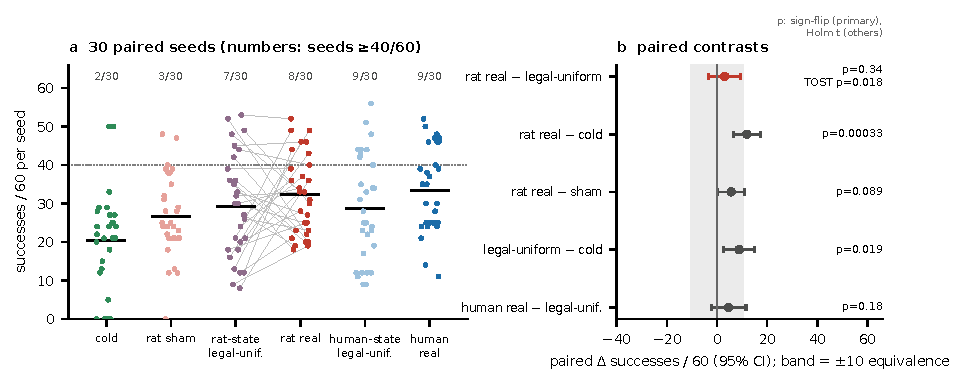
\includegraphics[width=\textwidth]{figs/fig_seeds30.pdf}
\caption{\textbf{E1: source-layout adaptation (30 paired seeds).} \textbf{a}~Successes out of 60 per seed with online PPO updates; lines
pair rat real with rat legal-uniform; numbers count seeds $\geq$40/60. \textbf{b}~Paired differences, 95\% CIs;
band = registered $\pm10/60$ equivalence margin (16.7 percentage points).}
\label{fig:seeds30}
\end{figure*}

\subsection{E3: sequential learning and replay}
\textbf{Protocol.} Copies of the source checkpoint learn room~A's goal (65,536 interactions), then room~B's goal in
the paired room (65,536 more), with PPO or replay; frozen probes follow each phase. E3 has a development pair (30 seeds)
and seven withheld pairs (15 seeds). Pairs were reserved before the development outcome; the crossed GPU repair was
registered after the original follow-up outcome. Rooms are visible and no task ID is supplied.
Forgetting is $F_s=S_{s,A}^{\text{after A}}-S_{s,A}^{\text{after B}}$, interpreted together with acquisition of B.

\textbf{Replay control.} A 620-entry reservoir stores experienced observations and their pre-update policy/value
predictions $(o,\tilde\pi,\tilde v)$~\cite{lin1992,rolnick2019}. After each PPO rollout update, one separate optimizer
step on up to 128 stored entries minimises
\begin{equation}
\mathcal L_{\rm replay}=\mathbb E_{\mathcal B}\!\left[
D_{\rm KL}(\tilde\pi\Vert\pi_\theta(\cdot\mid o))
+\tfrac14(V_\theta(o)-\tilde v)^2\right].
\label{eq:replay}
\end{equation}
New rollout entries enter the reservoir afterwards; it samples experience across A and B without a boundary signal.
This is a replay baseline, not a new memory rule, and incurs extra storage and optimizer steps.

\begin{figure*}[t]
\centering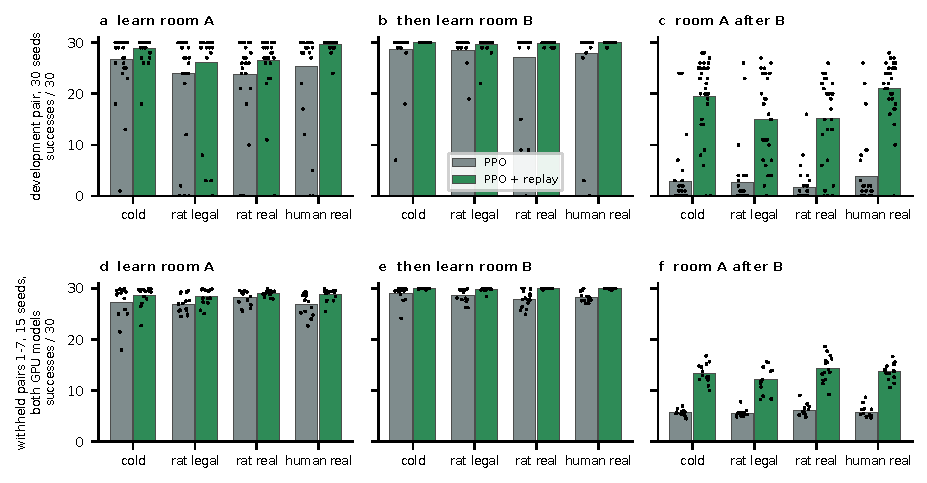
\includegraphics[width=\textwidth]{figs/fig_continual.pdf}
\caption{\textbf{E3: sequential learning in visible rooms.} Agents learn room~A's goal (65,536 interactions), then
room~B's goal in the paired room (65,536 more), with no task signal; frozen probes, 30 trials each. Grey: PPO;
green: PPO with a 620-transition policy/value replay buffer. Bars are seed means, dots are seeds. \textbf{a--c}~development pair, 30 seeds (both methods of each seed on the same GPU model); \textbf{d--f}~seven
withheld pairs, 15 seeds, each value averaged over pairs and both GPU models (crossed follow-up).}
\label{fig:continual}
\end{figure*}


\textbf{E3: forgetting is catastrophic without replay; replay reduces it under every tested prior (Fig.~\ref{fig:continual}).}
On the development pair (30 seeds), both methods learn A and B, but PPO retains only 1.7--3.8/30 successes
on A after learning B; replay retains 14.9--20.9. Replay reduces forgetting by $11.9/30$ ($[9.8,14.1]$), within
every prior (Holm $p\leq.00012$). These method contrasts are hardware-matched. Prior-versus-cold and rat
real-versus-legal contrasts are confounded with GPU model and are not interpreted.
After B, PPO paths in A concentrate on B's goal location; replay paths return to A's goal
(supplement). This is descriptive evidence of interference, not an identified internal mechanism.

\textbf{Withheld room pairs.} Seven pairs were reserved before the development outcome. The original follow-up
confounded method and GPU model; a repair registered after seeing that result added 840 complementary fits, crossing
all methods, priors, pairs and seeds with both GPU models. With pairs and hardware averaged within 15 seeds,
PPO retains 5.6--6.1/30 and replay 12.2--14.4. Replay reduces forgetting by $6.2/30$ ($[5.1,7.4]$, $p=2\times10^{-8}$),
within every prior and on both GPUs (6.2 and 6.3), about half the development effect. The method$\times$hardware
interaction lies within $\pm$10 percentage points (TOST $p=.0002$).
Prior-versus-scratch differences in A acquisition, and human-versus-rat differences in forgetting, lie within that
same margin; smaller effects remain compatible. The supplement gives secondary contrasts and execution history.


\textbf{Learning curves (registered, 10 seeds).} A further hardware-matched sequential study finds no resolved
new-goal learning-curve advantage: human versus legal $+14$ points ($[-6,35]$), versus scratch $-16$
($[-34,3]$; Holm $p=.17$ for both). The acquisition gate passes (25.5--29.7/30 on the new goal), and replay
again retains more of the first goal ($+14.9/30$, $[10.3,19.5]$). Curves and protocol are supplementary.

\textbf{Task-addressed protection (exploratory).} On one development pair, Nevo-CRL-inspired
PPO masking~\cite{li2026nevo} retains 22--30/30 first-goal successes while acquiring B at 18--30/30;
task-ID PPO retains 0--6/30 (three seeds). Task-routed recurrent-residual agents also retain A while acquiring B (3/3 seeds; supplement). Both pilots use backpropagation and provided task IDs; neither is a native reproduction or
local-learning result.

\subsection{Predicted cortical responses as visual input}
\textbf{Predicted cortical responses.} We also refit the camera-only experiment using a frozen model of mouse
visual cortex~\cite{wang2025fnn}, or a randomized core retaining the trained readout, perspective and modulation.
The model predicts responses of 9,941 neurons to the agent's own reconstructed frame; these are not recordings
during navigation. PCA to 144 features uses source layouts 0--5 only. All three perceptions meet the source
competence rule (10 new paired seeds). In the 16 exposed rooms, human choices exceed legal labels by 11.5 points
with pixels, 3.7 with predicted responses, and 0.7 with the randomized core; none resolves under the registered
Holm correction ($p=.135,.508,.775$; Fig.~\ref{fig:microns}). These estimates do not establish differences in
prior benefit across perceptions. The mouse model also sees higher-resolution frames than the pixel policy;
this sensitivity test establishes neither neural superiority nor transfer from measured neural activity.

\begin{figure}[t]
\centering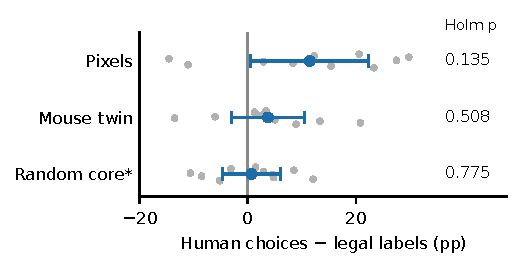
\includegraphics[width=\linewidth]{figs/fig_microns_prior.pdf}
\caption{\textbf{Changing the visual representation} (10 paired seeds, 16 exposed rooms). Dots: seeds;
blue: means and unadjusted 95\% CIs. Registered exact tests use Holm correction over the three perceptions.
The mouse model uses predicted responses. *Randomized core retains a trained readout, perspective and modulation.}
\label{fig:microns}
\end{figure}

\subsection{Representation alignment (Rosetta)}
\begin{figure*}[t]
\centering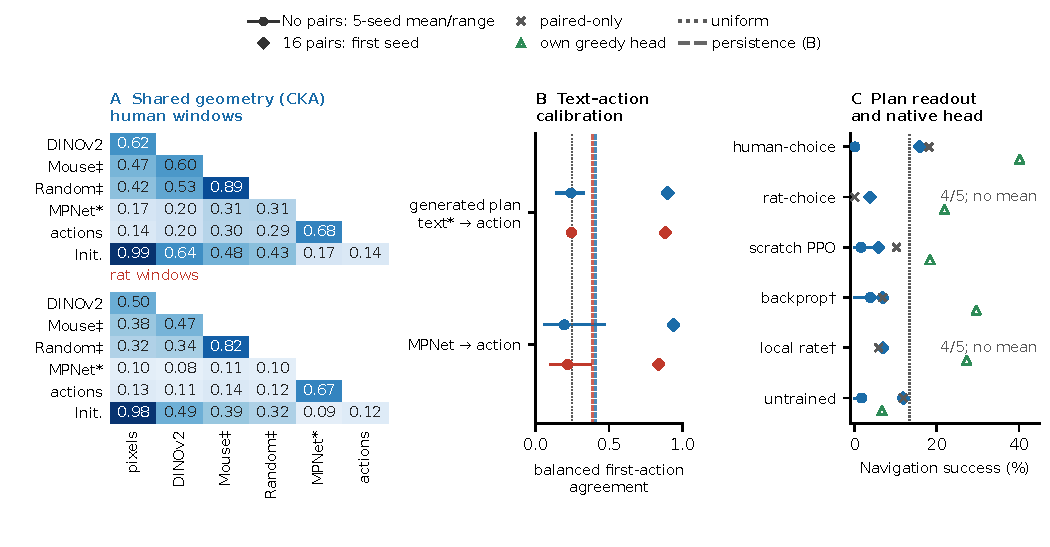
\includegraphics[width=\textwidth]{figs/fig_rosetta_main.pdf}
\caption{\textbf{Shared geometry, calibrated readout and acting.} \textbf{A}~Unbiased linear CKA (scale 0--1) on
292 human and 189 rat windows; every shown pair exceeds its 100-shuffle range. Init.: untrained policy.
\textbf{B}~Generated plan text mapped to actions: human (blue), rat (red); 16 anchors calibrate this constructed
correspondence. \textbf{C}~Plan maps versus each policy's own greedy head in 16 exposed rooms; uniform succeeds
at 13.3\%. Zero-pair means/ranges require five complete alignment seeds; 16-anchor and paired-only fits use the
first seed. *Text describes the plan. $\ddagger$Predicted mouse responses and partly trained random core.
$\dagger$Source continuations after a backprop warm start, with Adam; no local-memory claim. One policy seed;
full controls and provenance in the supplement.}
\label{fig:rosetta}
\end{figure*}



\textbf{Exploratory representation study.} Do transferable decisions also admit a common geometric readout?
Following Schnaus et al.~\cite{schnaus2026rosetta}, we apply their released Wasserstein--Procrustes aligner,
without modifying its equations, to frozen visual features, policy states and four-move plans.
We extract 5,674 windows from the recorded paths; fitting uses three disjoint 192-window source sets
(96 per species), separated by trial and camera frame, with 16 separate paired anchors for calibration.
Evaluation uses 481 windows from source layouts 6--7 (189 rat, 292 human; three rats, six humans).
These layouts were already exposed in earlier project evaluations: this is an exploratory follow-up.
Plans are 16-dimensional concatenated one-hot actions, not an action foundation model; text is a generated
description of the same plan. Visual encoders include pixels, DINOv2~\cite{oquab2023dinov2}, predicted mouse responses and the random
core; language encoders are MiniLM~\cite{wang2020minilm} and MPNet~\cite{song2020mpnet}. Policy states are action-trained, not unimodal action pretraining.

\textbf{Geometry and calibration.} We measure source-centred, row-normalised unbiased linear CKA between
representations on the same evaluation windows, separately by recorded species; 100 row shuffles give
descriptive references, not tests over independent animals. DINOv2--MPNet, DINOv2--action and MPNet--action
CKAs are .20/.20/.68 on human windows and .08/.11/.67 on rat windows, all above their shuffle ranges.
All 132 pairs exceed these descriptive ranges, including untrained controls: similarity does not establish
learned convergence or cortex-specific structure (Fig.~\ref{fig:rosetta}). With 16 anchors, generated-text-to-plan alignment reaches 88.4\% balanced first-action
agreement on rat windows and 89.9\% on human windows; MPNet gives 83.7\% and 93.9\%. This is calibrated
correspondence for constructed commands, not independently acquired language grounding. Without anchors, all
14 complete five-seed primary group means trail action persistence (.388 rat, .409 human).
Image--history and text--history combinations do not consistently improve on matched history-only references.

\textbf{Closing the action loop.} Alignment uses five fixed algorithm seeds, 0 or 16 pairs, and a paired-only
Procrustes reference; incomplete groups have no mean. At each agent-generated view, we retrieve from all
256 plans and execute the first action, splitting probability uniformly over tied top plans before replanning.
In the same 16 exposed rooms, the human-trained policy's greedy head succeeds on 40.2\% of trials;
its unpaired action/text readouts average 0.08\%/8.38\%, and the 16-anchor readouts reach 15.8\%/15.2\%.
Some calibrated maps improve over matched untrained maps, but all 68 evaluated trained-policy maps remain
below their own greedy heads. This acting comparison uses one policy-training seed and one evaluation seed;
alignment seeds measure optimizer variability. Shared structure, calibrated readout and useful navigation
are distinct tests. These results do not establish universal cross-species representations or a limitation
of the original common-content image--text setting.
\FloatBarrier


\section{Figures moved from the main paper for space}
\label{sec:movedfigs}
\begin{figure*}[t]
\centering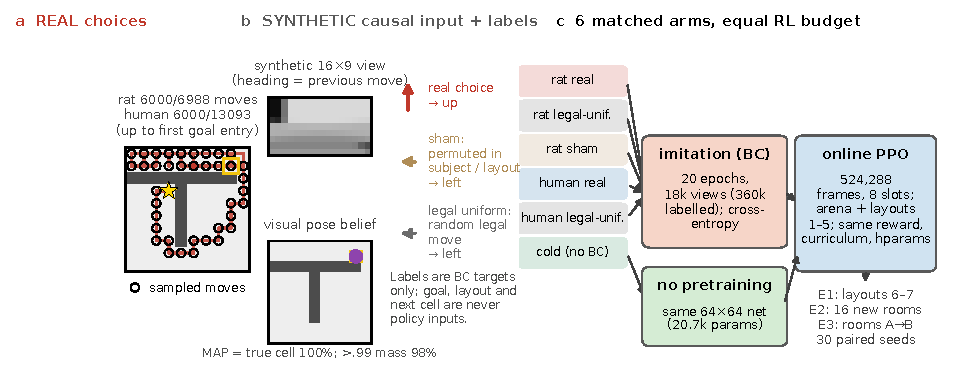
\includegraphics[width=\textwidth]{figs/fig_prior_pipeline.pdf}
\caption{\textbf{From recorded paths to acting agents.} Recorded cell-to-cell moves supply labels; views and pose
beliefs are reconstructed causally from the path prefix (never from the label being predicted). Control arms keep the
same observations and replace the labels. All arms then receive the same 524,288 reinforcement-learning interactions.}
\label{fig:pipeline}
\end{figure*}
\begin{figure}[t]
\centering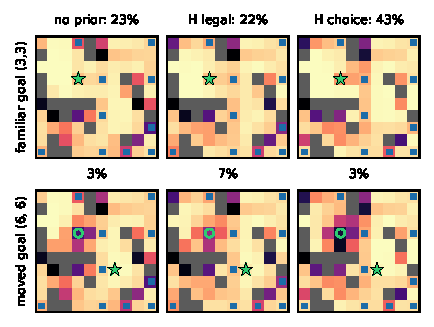
\includegraphics[width=\linewidth]{figs/fig_camera_paths.pdf}
\caption{\textbf{Where frozen agents go} in one fresh room (chosen before viewing; 30 seeds $\times$ 30 trials per
arm). Shade: visits per trial (log); grey: walls; squares: starts; star: goal; circle: familiar goal. Titles: success.}
\label{fig:paths}
\end{figure}
\FloatBarrier

\section{Provenance and independent audits}
Each study records a protocol before its own outcomes; post-result follow-ups state which earlier outcomes were known.
Audits used a separate agent with its own scripts, sharing registered helpers, except for the author audits identified
in Table~\ref{tab:prov}. Checks cover records, checkpoint/data bindings, physical paths and statistics; specified
first-seed checks re-execute physics, rendering, the pose filter and frozen-policy probabilities from logged actions.
This is computational verification within the study, not external experimental replication.

\begin{table}[h]\centering\small
\begin{tabularx}{\linewidth}{>{\raggedright\arraybackslash}p{3.4cm}>{\raggedright\arraybackslash}p{2.6cm}>{\raggedright\arraybackslash}X>{\raggedright\arraybackslash}p{3.3cm}}
\toprule
study & registration & checked independently & first-seed re-execution\\\midrule
E1 transfer (30 seeds) & before outcome & all selection episodes replayed & all E1 selection episodes\\
E2 zero-shot rooms (30 seeds) & before outcome & aggregates and statistics of all 2,880 probes & 96 probes\\
E3 continual, development pair & before outcome & all bindings and statistics & first-seed runs of every cohort\\
E3 crossed withheld-pair follow-up & pairs before; GPU repair after original outcome & all crossed bindings and statistics & first-seed runs of all four cohorts\\
E2 expert/surrogate follow-up & after main E2 result & 120 source budgets, 1,920 probe aggregates, statistics & 64 probes\\
GPU counterbalance & after main E2 result & 90 source budgets, 1,440 probe aggregates, statistics & 48 probes\\
Entropy-matched expert & after main E2 result & 60 calibrated checkpoints, 960 probe aggregates, statistics & 32 probes\\
Grouped-individual refits & after main E2 result & 120 source fits, 1,920 probe aggregates, statistics & 192 probes\\
Input ablation & after main E2 result & 90 source fits, 13,500 source and 1,440 target probes, statistics & 144 masked-policy probes\\
All-optimal expert & after main E2 result & 10 teacher fits, 10 calibrations, 320 probes, statistics & 32 probes\\
Fresh-room confirmation & before geometry and outcome & geometry, 3,680 probes, statistics & 176 room blocks\\
Perturbed and denser rooms & before any fresh outcome & dense geometry, 7,200 probes, statistics & 240 blocks\\
Mechanism (label interventions) & post-result follow-up on fresh rooms & 8 label sets, 80 source fits, 1,280 probes, statistics & 128 blocks\\
Dose response & before fits and outcome & 80 source fits, 1,280 probes, statistics & 128 blocks; first-seed BC re-run\\
Appearance and capacity & before rooms and outcome & 30 wide source fits, 9,120 probes, statistics & 432 blocks with own view changes\\
Brightness augmentation & after the dimming outcome, before any fit & all 120 fits and 5,760 probes, statistics (study authors) & 6 first-seed refits (bit-exact), 288 blocks (exact)\\
Learning curves and retention & before any fit & all 60 fits: training observations, rewards, paths, checkpoints, probes; statistics and gate & first-unit frozen action probes\\
Rosetta alignment/acting & before each fit/probe; pairwise after acting & all 176 completed fit metrics; all 132 pairwise CKAs and 13,200 shuffles & 75,840 acting episodes, all available map parities\\
Mouse-model inputs & before any fit & all 90 fits, 13,500 source trials, 1,440 room blocks; checkpoints, paths and statistics & 2 trials for every arm/input at seed 1300 (9 exact GPU replays)\\
Task-addressed protection pilot & corrected code bound after invalid development outcomes & all six source/checkpoint bindings, native protection masks, microstep logs & all 540 frozen episodes, explicit CPU forward replay\\
FF + recurrent residual & after failed acquisition; before new fits & all six cases, initial weights, protection and recurrent updates & all 540 frozen episodes, explicit matrix replay\\
\bottomrule
\end{tabularx}
\caption{\textbf{Study provenance.} ``After main E2 result'' denotes exposed-room follow-ups.
Dose and brightness studies used separate author-written pre-probe audits; the independent auditor later
checked the complete dose cohort, reproducing its analysis to $3\times10^{-16}$.
The first wide-network probe launch stopped at checkpoint loading, before outcomes, because the shared builder
fixed the width; a separate launcher set the registered width and the unchanged probe code ran.}
\label{tab:prov}
\end{table}

\paragraph{Numerical tolerances.} Re-executed frozen-policy probabilities match within $10^{-5}$. Behaviour-cloning
re-runs across processes on the same GPU model differ only by floating-point noise (parameters $\leq3\times10^{-5}$,
action probabilities $\leq5\times10^{-6}$, argmax agreement 100\% on all 18,000 source views); within one process they
are identical.

\section{Agent architecture and learning rules}
\begin{figure}[ht]
\centering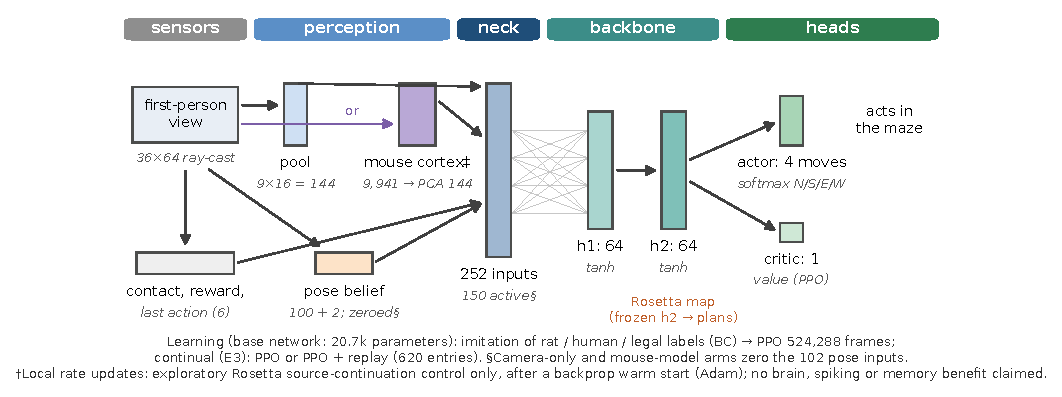
\includegraphics[width=\linewidth]{figs/fig_v4n_architecture.pdf}
\caption{\textbf{Base architecture.} The 20.7k-parameter policy receives a pooled camera or frozen visual-model
features, public feedback and a visually derived pose belief. Camera-only and mouse-model conditions zero the
102 belief-derived inputs. $\ddagger$Mouse features are model predictions, not recordings. The actor and critic are
trained with PPO; E3 adds the stated replay control. Exploratory local-rate Rosetta continuations start after
backpropagation training and use Adam; they do not demonstrate spiking or memory protection. The larger-network
capacity follow-up uses a separate $256\times256$ backbone.}
\label{fig:architecture}
\end{figure}

\section{Descriptive E1 occupancy}
Human choices increase agents' occupancy correlation with the human reference relative to legal actions at the same
states ($+.063$ $r$, 95\% bootstrap CI $[.026,.098]$), whereas rat choices do not resolve an increase in correlation
with the rat reference ($+.004$, $[-.029,.038]$). These spatial correlations do not identify an internal mechanism.
\begin{figure}[ht]
\centering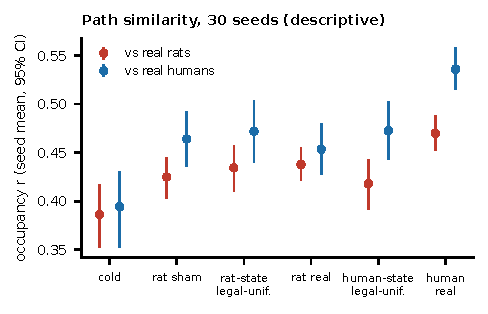
\includegraphics[width=.52\linewidth]{figs/fig_seeds30_alignment.pdf}
\caption{\textbf{E1 paths (descriptive).} Seed-mean occupancy correlation with recorded rats and humans on layouts
6--7; 95\% bootstrap intervals over 30 training seeds.}
\end{figure}

\section{Predicted mouse cortical responses as visual inputs}
This follow-up was registered after the behavioural E2 results and before any of its 90 fits. It uses the released
mouse visual-cortex predictor~\cite{wang2025fnn} with the scan 8--5 readout (9,941 units). Responses are predictions
on the agent's reconstructed views, not neural recordings acquired during navigation. Each 36$\times$64 luminance
frame is gamma encoded ($1/2.2$), upsampled fourfold by nearest neighbour, and presented as a separate clip of ten
grey frames followed by fifteen repetitions of the current view. We average the last ten predicted responses.
This assumes a monitor geometry and uses repeated static views, rather than a measured animal visual stream; the
encoder is not presented with future actions or views. The random-core control retains the trained readout,
perspective and modulation, so it is partly pretrained. Pixels use the original 9$\times$16 pooled camera, whereas
both model conditions use the full 36$\times$64 frame; visual information and pretraining are not matched.

PCA is fitted on 4,616 unique frames from source layouts 0--5 only. The 144 components are scaled by source standard
deviations and clipped to $[-1,1]$ after division by three. Layouts 6--7 and the 16 exposed rooms are transformed
without fitting. A policy-input hook replaces only the 144 camera channels for imitation, PPO and frozen evaluation;
public feedback is retained and the 102 belief-derived channels remain zero. Exact pooled-frame keys identify the
same full frames in the fixed benchmark. Precomputed features preserve the frozen encoding function; no inference
latency, energy, spiking or deployability claim is made.

The three label arms (human choices, legal labels at the same human states, and no imitation) are refitted for all
three inputs at ten new paired seeds (1300--1309), with the original imitation and 524,288-interaction PPO budgets.
All inputs pass the source rule: at least 75/150 successes in at least eight seeds for each arm. The 16 previously
exposed E2 rooms supply 30 frozen trials per room and seed, so this is a sensitivity study, not fresh confirmation.
The registered primary contrast is human minus legal, with an exact two-sided sign-flip test and Holm correction
over three inputs; unadjusted $t$-intervals are descriptive. None resolves (Table~\ref{tab:microns}). Differences in
significance do not establish an interaction between input and prior. The independent audit checks all 90 source
checkpoints and 43,200 target episodes and exactly replays two trials in each of the nine arm/input cells at seed
1300 on its original GPU. Earlier audit-code assumptions about inference counters, source-record fields and CPU
versus GPU roundoff were corrected with previous code/logs preserved; no scientific fit or outcome was changed.

\begin{table}[ht]\centering\small
\begin{tabular}{lrrrcc}
\toprule
input & human & legal & scratch & human $-$ legal, points [95\% CI] & Holm $p$\\\midrule
Pixels & 15.66 & 12.22 & 11.24 & $+11.46$ [$0.53,22.39$] & .135\\
Mouse model & 13.41 & 12.29 & 12.13 & $+3.73$ [$-3.10,10.56$] & .508\\
Random core & 14.18 & 13.97 & 12.34 & $+0.69$ [$-4.60,5.97$] & .775\\
\bottomrule
\end{tabular}
\caption{\textbf{Changing the visual encoding.} Mean successes out of 30, averaged over 16 rooms and ten paired
training seeds; paired differences in percentage points. CIs are unadjusted. Holm corrects the three registered
exact tests. All three inputs pass source competence; the effect of the human prior remains unresolved here.}
\label{tab:microns}
\end{table}

\section{Fresh-room gains: seed and room uncertainty (post hoc)}
The registered fresh-room tests treat the 30 (or 10) training seeds as the unit and average each seed over the same 16
rooms. To check that the gains are not driven by a few rooms, a post-hoc sensitivity analysis (not a new primary test;
registered tests unchanged) resamples seeds, rooms, or both together, with replacement and keeping each human/control pair
intact (10,000 resamples; percentile intervals, approximate). Table~\ref{tab:crossed} gives successes out of 30 per room.
Rooms come from one constrained generator and the same source-trained policies, so this addresses room-to-room
variation within that generator, not animals, species populations or real-world tasks. The study's authors
recomputed every mean and count from the audited probe records and reproduced the intervals with an independent
resampler (differences $\leq0.1$ success).
\begin{table}[h]\centering\small
\begin{tabular}{lrrccccr}
\toprule
contrast & seeds & mean & seeds only & rooms only & crossed & crossed, Bonf.\,4 & rooms $>0$\\\midrule
Full input: human $-$ legal & 30 & $+2.97$ & [2.1, 3.8] & [2.0, 3.9] & [1.6, 4.4] & [1.2, 4.8] & 16/16\\
Full input: human $-$ scratch & 30 & $+3.66$ & [2.7, 4.6] & [1.7, 5.5] & [1.4, 5.8] & [0.7, 6.4] & 13/16\\
Camera only: human $-$ legal & 10 & $+4.55$ & [2.2, 6.8] & [3.0, 6.1] & [1.6, 7.4] & [0.8, 8.2] & 15/16\\
Camera only: human $-$ scratch & 10 & $+6.68$ & [5.2, 8.3] & [5.0, 8.5] & [4.2, 9.1] & [3.5, 9.8] & 16/16\\
\bottomrule
\end{tabular}
\caption{\textbf{Fresh-room gains under seed, room and crossed resampling} (post hoc). Intervals are 95\% percentile
bootstrap intervals; ``Bonf.\,4'' is a nominal 98.75\% interval for the four contrasts. Rooms $>0$: rooms whose
seed-averaged gain is positive.}
\label{tab:crossed}
\end{table}

\section{Dose and brightness curves}
\begin{figure}[ht]
\centering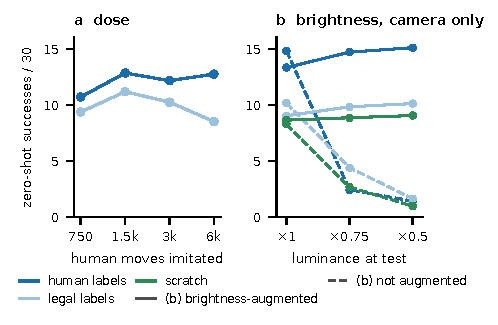
\includegraphics[width=.67\linewidth]{figs/fig_dose_light.pdf}
\caption{\textbf{Dose and brightness sensitivity.} Descriptive means from the audited records. Left: 10 paired seeds,
16 new rooms; only the full-dose human--legal contrast is resolved after Holm correction, and the registered
log-dose trend is unresolved ($p=.09$). Right: camera-only agents, 20 paired seeds, 16 rooms. Solid: training gains
uniform in $[0.5,1]$ per episode; dashed: no brightness augmentation. Both dimmed tests lie within the augmentation
range. These panels add no experiment or inferential test.}
\end{figure}

\section{Decision-feature interventions}
\begin{figure}[t]
\centering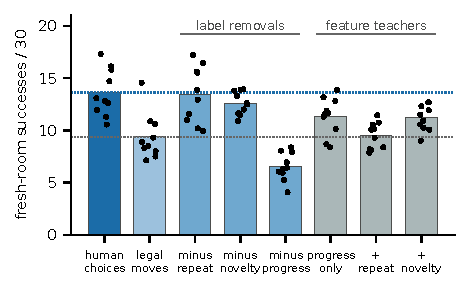
\includegraphics[width=\linewidth]{figs/fig_mechanism.pdf}
\caption{\textbf{Decision-feature interventions} (post-result follow-up on the fresh rooms; 10 seeds, all trained
in one code path on one GPU model). Bars: seed means; dots: seeds; dotted lines: human and legal labels. Removals
replace, where a matched alternative exists, human moves that have the feature by otherwise matched moves that lack
it; teachers sample labels from conditional-logit models fitted to the human source moves.}
\label{fig:mechanism}
\end{figure}
\section{Detailed E2 follow-ups}
These details retain the full contrasts behind the compressed main-paper results. The order below follows the original study sequence; fresh-room confirmation reuses policies, not outcomes or fitted parameters.

\paragraph{Feature teachers.} For recorded state $x$ and candidate action $a$, the three binary features $f(x,a)$
indicate repeating the previous move, reducing shortest-path goal distance and entering a cell not yet visited in the
recorded trial. Source-only conditional-logit fitting uses
\begin{equation}
q_\beta(a\mid x)=\frac{\mathbf 1[a\in\mathcal A_{\rm legal}(x)]\exp(\beta^\top f(x,a))}
{\sum_{a'\in\mathcal A_{\rm legal}(x)}\exp(\beta^\top f(x,a'))}.
\end{equation}
The fitted teacher samples replacement labels; it is not available to the agent at inference. Geometry and goal
distance are privileged offline supervision for these controls. No target-room actions are used for fitting.

\textbf{E2: human choices generalise to unseen rooms (main-paper E2 figures).} Mean zero-shot
successes out of 30 are 9.7 (cold), 9.1--9.9 (rat sham/legal/real), 10.3 (human legal) and 13.3 (human real). Only
human real beats cold ($+3.6$, Holm $p=9\times10^{-7}$) and legal moves at the same human states ($+3.0$,
$p=8\times10^{-8}$), so visited states alone do not explain the gain. Rat real is equivalent to rat legal (TOST
$\pm3/30$, $p=2\times10^{-7}$); an exploratory dataset (species/apparatus)$\times$choice interaction is $+2.8$ ($[1.5,4.2]$,
$p=1.2\times10^{-4}$). \textbf{Relabelled states.} A follow-up registered after this result relabels the same
human states. Run on both GPU models (no label$\times$hardware interaction beyond $\pm$10 points, TOST $p\leq.001$),
human choices beat a shortest-path expert by $+4.4$ and a fitted persistence-plus-goal model by $+2.2$ (Holm
$p=1\times10^{-13}$, $3\times10^{-7}$). The expert scores 9.0/30 (scratch 9.7; not tested). Matching its mean source
entropy to the human agent's with a global temperature leaves it 4.6 below ($p=3\times10^{-15}$). It breaks ties by a
fixed direction order (44\% of sampled decision points have several optimal moves), so a further follow-up (input-study
seeds) trains on soft targets spread equally over \emph{all} optimal moves: after the same temperature matching, human
choices still beat it by $+3.2$ ($[1.8,4.5]$, $p=5\times10^{-4}$, unadjusted as registered; raw teacher $+2.5$,
descriptive; full input, previously exposed rooms). This addresses the tie-break concern without exhausting all
expert policies; soft labels carry more information per row, only mean source entropy is matched, and state-wise and
out-of-distribution confidence are untested. \textbf{Grouped-individual
refits.} Refits on three folds that each withhold a third of the individuals (half the dose, 10 new seeds)
keep human real above legal ($+2.8$, Holm $p=1\times10^{-4}$, positive in 10/10 seeds and 3/3 folds); rat is
unresolved ($+0.6$). Withheld individuals are absent from prior training, but tests are in the same exposed digital rooms, not on new individuals.
\textbf{Inputs.} Retraining all arms with channels zeroed (10 new seeds) shows that the advantage does not need
the calibrated place belief. With pixels and feedback alone, human choices beat legal by $+4.3$ and scratch by
$+7.3$ (Holm $p=.03$, $5\times10^{-5}$ over 8 contrasts), as with full input ($+4.2$, $p=.004$). Without direct
pixels (the place belief is still visually derived) the gain is unresolved ($+2.4$, Holm $p=.08$). Neither interaction is resolved or equivalent, so we claim
neither that pixels are required nor that benefits are identical. Training and the matched probes still run the place
observer, but a frozen re-execution of all camera-only arms (seed 1200, 16 rooms, 1,440 episodes) with the observer
disabled reproduces every action and path exactly, so it is not needed at inference (no runtime or energy claim).
\textbf{Fresh-room confirmation.} All analyses above reuse the same 16 rooms. Registered before any outcome, the
same frozen policies were therefore probed in 16 newly generated rooms that no experiment, analysis or design choice
had touched (same generator rules, new seed; 3,680 probes). Everything replicated (the main-paper control figure, open
markers): human choices beat legal moves by $+3.0$ ($[2.1,3.9]$) and scratch by $+3.7$ ($[2.6,4.7]$; Holm
$p\leq3\times10^{-7}$); rat choices stayed equivalent to legal moves ($+0.3$, TOST $p=7\times10^{-6}$); the
dataset$\times$choice interaction, exploratory above, was confirmed ($+2.7$, $[1.4,4.1]$, $p=3\times10^{-4}$);
camera-only human choices beat legal moves by $+4.6$ and scratch by $+6.7$ (Holm $p=.005$, $4\times10^{-5}$); and
full-input human choices beat the calibrated all-optimal expert by $+3.1$ ($p=.007$). A post-hoc bootstrap that resamples seeds and rooms together keeps all four human gains above zero (e.g.\ $[1.6,4.4]$ over legal moves), and the full-input gain over legal moves is positive in all 16 rooms (Table~\ref{tab:crossed}).
\textbf{Perturbed and denser rooms.} Also registered before any fresh outcome, the same policies faced pixel noise
(which also enters the visual place belief), denser rooms (26 instead of 18 walls; detours three times longer) and
both (the main-paper robustness figure). Density lowered every arm's success; noise, unexpectedly, raised it for every arm, so it
is a sensory perturbation rather than added difficulty. Under all three conditions human choices beat legal moves and
scratch (Holm $p\leq2\times10^{-5}$ over 6 contrasts), and rat choices stay equivalent to legal moves (TOST
$p\leq10^{-4}$). These are variants of the same grid task, not a richer or real-world benchmark.
\textbf{What in human choices transfers?} A post-result, source-only follow-up on the fresh rooms (10 seeds, one
training code path; Fig.~\ref{fig:mechanism}) edits the human labels, or replaces them with teachers built from three
decision features computed from the recorded paths: repeating the previous move, moving closer to the goal and
entering an unvisited cell (humans .49, .77 and .92 of moves; legal-move chance .25, .45 and .65). Human labels beat
legal moves by $+4.3$ ($p=4\times10^{-4}$). Replacing goal-progress moves with otherwise matched non-progress moves
(25\% of labels) cut success by 7.1 (Holm $p=3\times10^{-5}$), below legal labels, whereas matched removal of
repetition ($+0.2$) or novelty ($+1.0$) was unresolved. A teacher sampling from all three features recovered only
part of the advantage: human labels still beat it by 2.4 ($p=.008$), leaving 57\% ($[32,87]$) of the human--legal gap
unexplained, although adding novelty to repetition and progress helped ($+1.7$, Holm $p=1\times10^{-4}$). These are
matched label interventions within this pipeline, not evidence about human cognition or a unique cause: goal-directed content contributes materially, and human choices carry
further transferable structure that these limited feature teachers do not capture.
\textbf{Dose.} Pretraining on nested subsets of 750, 1,500, 3,000 or 6,000 human moves with equal training (10 new seeds,
16 further new rooms; registered) gave human--legal advantages of $+1.3$, $+1.7$, $+1.9$ and $+4.2$. Only the full dose
was resolved (Holm $p=.007$), replicating the main result once more; the registered log-dose trend ($+0.9$ per doubling,
$[-0.2,2.0]$, $p=.09$) was unresolved, and part of the widening gap reflects legal-label agents declining at the largest
dose (descriptive).
\textbf{Appearance and capacity.} Registered before any outcome, the frozen policies were probed in 16 further new
rooms with altered wall and floor texture, or with all rendered luminance scaled by 0.75; separately, the human,
legal and scratch arms were retrained with a 6.4$\times$ larger network ($256\times256$ hidden units; 10 new seeds;
9,120 probes, independently audited; the main-paper robustness figure, right). With new textures human choices still beat legal
moves and scratch ($+3.1$, $+3.8$; camera-only $+4.4$, $+6.9$; Holm $p\leq.009$ over 10 contrasts), and so did the larger network
($+4.5$, $+4.0$; Holm $p=.019$), a capacity replication in the same pipeline rather than a new architecture.
Dimming, however, lowered every arm (human choices 12.4 to 4.8/30; camera-only 15.1 to 2.1) and the human advantage
was not detected (full input $+0.3$, $-1.4$; camera-only $-3.2$, $-2.4$; Holm $p\geq.21$, unresolved, not equivalence).
No agent had been trained with photometric augmentation. A follow-up registered after this outcome but before any
fit (camera-only, 20 new seeds, 120 fits, 5,760 probes) retrained all three arms with and without a random brightness
gain per episode ($\times$0.5--1, training only). Without it, dimming again collapsed every arm (human choices 14.8
to 2.4/30); with it, success held (14.7/30 at $\times$0.75) and human choices beat legal moves and scratch by $+4.9$
and $+5.9$ at $\times$0.75 (Holm $p\leq2\times10^{-5}$) and by $+5.0$ and $+6.1$ at $\times$0.5; augmentation widened the
human--legal gap under dimming by $+6.9$ ($[4.8,8.9]$, Holm $p=2\times10^{-6}$). Both levels lie within the training
range, so this shows robustness under standard augmentation, not extrapolation.
Rat choices stayed equivalent to legal moves under all three views (TOST $p\leq.002$).

\section{Sequential-learning controls}
On the development pair, PPO learns room~A (23.7--26.7/30) and room~B ($\geq$27/30) but then succeeds on only
1.7--3.8/30 room-A trials, although the rooms are visually distinguishable from the first view in most starts.
Replay keeps 14.9--20.9/30 while learning~B ($\geq$29.6/30). With seeds as units (arms averaged within seed),
replay reduces forgetting by 11.9/30 ($[9.8,14.1]$, $n=30$, $p=3.5\times10^{-12}$), and by 10.0--14.3 within every
prior (Holm $p\leq1.2\times10^{-4}$). Each prior's two methods ran on the same GPU model, so these within-prior contrasts are hardware-matched;
comparisons between priors are not, except human versus rat (same GPU), which show no resolved difference in acquisition
or forgetting (not tested for equivalence here). Prior-versus-cold and rat real-versus-legal contrasts in E3 are confounded with GPU model and not
interpreted. The paths show what is lost (Fig.~\ref{fig:forgetpaths}): after
learning~B, PPO agents placed in room~A converge on the cell where room~B's goal lies, consistent with
interference from the newer goal rather than undirected search; occupancy alone does not show which internal
representation changed. Replay agents return to room~A's goal.
\textbf{Crossed withheld-pair follow-up} (seven pairs, 15 seeds, the main-paper sequential-learning figure, panels d--f). The original run
confounded method with GPU model (every PPO fit on one model, every replay fit on the other); we therefore ran the
complementary 840 fits so that every method, prior, pair and seed exists on both models, and average per seed. This
crossed design was registered after the confounded outcome had been seen. PPO keeps 5.6--6.1/30 of room~A after
learning~B; replay keeps 12.2--14.4. Replay reduces forgetting by 6.2/30 ($[5.1,7.4]$, $n=15$, $p=2\times10^{-8}$),
on each GPU model (6.2 and 6.3), within every prior (5.1--7.3, Holm $p\leq2\times10^{-5}$) and on all seven pairs
(sign test $p=.016$; small on two), with no method$\times$hardware interaction beyond $\pm$10 percentage points
(TOST $p=.0002$). The effect is about half that on the development pair. With hardware balanced, prior-versus-scratch differences in
room-A success at the end of A learning lie within the registered $\pm$10-percentage-point margin (TOST $p\leq.004$);
smaller effects remain compatible. Rat real exceeds rat legal by $+0.9/30$ ($[0.2,1.6]$, unadjusted $p=.02$, a
registered secondary contrast) while also lying within that margin; human and rat priors are equivalent in
forgetting within the margin. One fit crashed (NumPy segmentation fault) and was rerun from its seed.

\section{Sequential-learning curves and spatial occupancy}
\begin{figure}[t]
\centering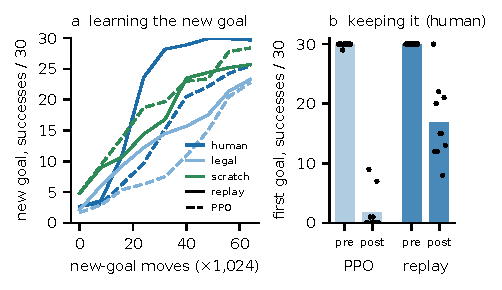
\includegraphics[width=\linewidth]{figs/fig_e4.pdf}
\caption{\textbf{Learning curves and retention} (registered; 10 seeds). \textbf{a}~Mean frozen-probe success on the
new goal during learning; primary tests compare priors within PPO (dashed). \textbf{b}~Human-prior agents' first-goal
success before and after learning the new goal; dots are seeds.}
\label{fig:e4}
\end{figure}
\textbf{Learning curves (registered).} Do human choices speed learning of a new goal (Fig.~\ref{fig:e4})? The main human, legal and scratch
source policies (10 seeds; all six prior$\times$method fits of a seed on one GPU model) kept their source goal in one
source layout for 65,536 moves, then learned a new goal in a second (65,536 more; frozen probes every 8,192). The area
under the new goal's learning curve showed no resolved prior effect: human versus legal $+14$ percentage points
($[-6,35]$), versus scratch $-16$ ($[-34,3]$; Holm $p=.17$ for both). Replay, interpreted only because the registered
acquisition gate passed (human agents reach 25.5--29.7/30 on the new goal), again retained more of the first goal
($+14.9/30$, $[10.3,19.5]$, Holm $p=1.4\times10^{-4}$; all 10 seeds), a hardware-matched replication of a known effect.




\begin{figure}[t]
\centering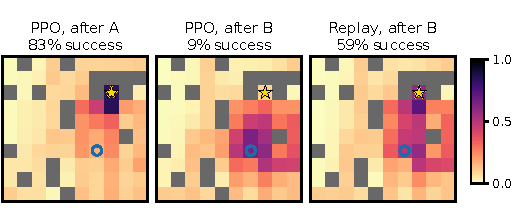
\includegraphics[width=\linewidth]{figs/fig_forgetting_paths_compact.pdf}
\caption{\textbf{Spatial occupancy before and after sequential learning.} Fraction of frozen room-A probe trials visiting each cell (development
pair; four priors $\times$ 30 seeds $\times$ 30 trials per panel). Grey: removed modules. After learning room~B, PPO
heads to B's goal location (circle); replay preserves visits to A's goal (star). Colour: trial fraction.
Descriptive aggregate; not a mechanism test.}
\label{fig:forgetpaths}
\end{figure}
\section{Task-addressed sparse-protection pilot}
\label{sec:nevo_pilot}
\begin{figure*}[t]
\centering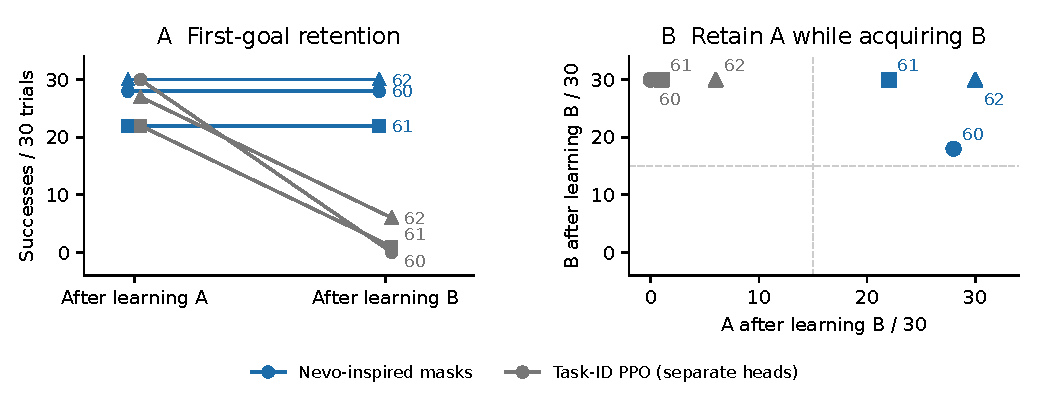
\includegraphics[width=.95\textwidth]{figs/fig_nevo_pilot.pdf}
\caption{\textbf{Exploratory task-addressed protection on one development room pair.} Each marker is one fixed
training seed (60--62); all six fits are shown. \textbf{A}~First-goal performance before and after learning B.
\textbf{B}~Retained first-goal and acquired second-goal performance; dashed lines mark 15/30 successes.
Both arms receive task identity. The masked policy preserves its A subnetwork exactly; this guarantee is
conditional on task-addressed routing. This is a backpropagation-trained Nevo-inspired adaptation, not a
verified native reproduction, an OOD test or evidence for local synaptic learning.}
\label{fig:nevo_pilot}
\end{figure*}
\paragraph{Question and scope.}
Can explicit subnetwork protection preserve a learned goal while another is acquired (Fig.~\ref{fig:nevo_pilot})?
Inspired by Nevo-CRL~\cite{li2026nevo}, we adapt task-specific neuron masks, training-rollout-based mask selection,
and hard freezing to the existing PPO pipeline. Native Nevo-CRL uses SAC, separate actors in its population,
semantic task-based reuse and different crossover/pruning rules. We have not reproduced its native benchmark;
this experiment tests an adapted protection mechanism. It uses backpropagation and is neither local nor spiking.
The original E3 experiment requires no task ID; this separate pilot supplies it during training and evaluation
to \emph{both} arms. It cannot establish an advantage over task-ID-free E3 or identify the contribution of
mask evolution separately from isolation and routing.

\paragraph{Design and deviations.}
Both arms start from the same rat-imitation/PPO source checkpoints for seeds 60--62 and learn the exposed E3
development pair (rooms 100 then 101). They use the same 64-unit two-layer body, 21,002 allocated parameters,
16 environments, PPO settings and 131,072 total environment interactions. Each nominal phase lasts 65,536 frames;
rooms switch at natural episode ends, so the first 127--322 phase-B frames still occur in A (exact per-case
exposures are bundled). Both arms reset Adam at B. The control has separate actor and critic heads selected
by task ID, with a shared plastic body. The masked arm uses one shared head and weight set, a population of
five masks, simplified importance-guided crossover and pruning every 32 PPO updates (16 evolutions total),
and training rollouts only for mask selection; search uses no additional interactions. Fitness is accumulated
rollout reward divided by terminal count, including unfinished-episode rewards, rather than exactly completed
episodic returns. Unlike native Nevo-CRL,
it has no semantic task encoder, separate population actors or exploration distillation. Initial A masks
sample half the units; B reuses the protected units and initially enables all remaining units.

For the saved A mask, first-layer active rows, second-layer active-pre/active-post intersections and head
columns are protected; active-unit biases and shared head biases are also frozen. Protected gradients are
zeroed before clipping, with an exact-restore assertion after \emph{each} Adam step. B can still change
unprotected weights. Inactive A-mask units remain masked during A evaluation. Thus preservation of the saved
A policy is guaranteed by construction when its task ID is supplied; it is not evidence that the agent infers
task boundaries or a biological mechanism.

\paragraph{Results and audit.}
The fixed competence gate requires A after A and B after B each to reach at least 15/30 successes in at least
two of three seeds, separately for each arm. All three seeds pass for both arms. For seeds 60/61/62, the masked
arm has A-before/A-after/B scores of 28/28/18, 22/22/30 and 30/30/30; the task-ID PPO control has 30/0/30,
22/1/30 and 27/6/30. These are descriptive results from one room pair, without confidence intervals or
population-level significance claims. Acquisition differs between arms; the result supports preservation
of each learned A policy, not faster learning or a general performance advantage.

An independent audit recomputes the native protection masks, verifies checkpoint hashes and zero protected
weight change, and replays all 540 saved evaluation episodes with an explicit CPU forward computation.
Action probabilities agree within $3.9\times10^{-7}$; all A paths and actions before/after B match in the masked
arm. Each masked fit logs 2,048 protected optimizer steps with zero drift even before restoration, while
unprotected weights change. The preserved A policy can therefore be distinguished from a policy that simply
stops all learning.

\paragraph{Execution history.}
An earlier six-fit implementation restored weights only after an entire PPO update, allowing protected entries
to drift between minibatches. Its outcomes were seen before independent review; those fits are invalid for
claims and are retained separately. The corrected code, sources, seeds, budget, gate and independent auditor
were bound before the six reported fits; no seeds were dropped or fits retried. Because the correction followed
exposed development results, this is a disclosed corrected pilot, not an independent confirmatory replication.

\section{Pretrained policy with a learned recurrent residual}
\label{sec:ffres_pilot}
\begin{figure*}[t]
\centering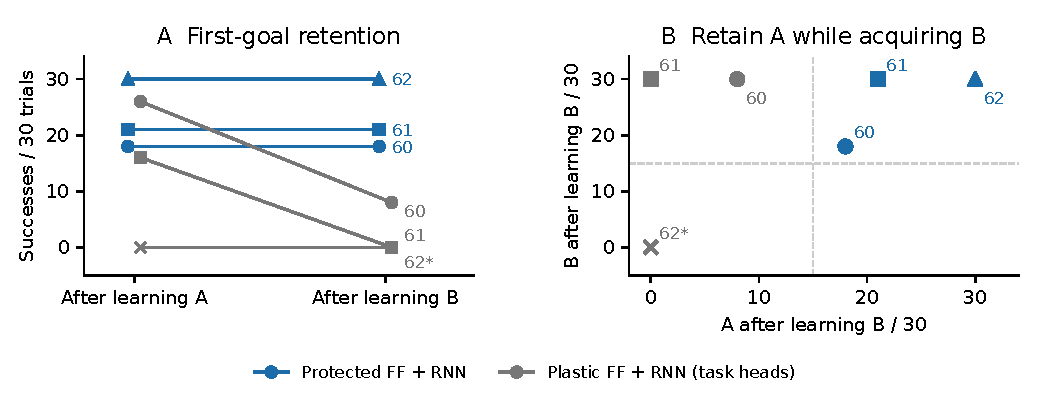
\includegraphics[width=.95\textwidth]{figs/fig_ffres_pilot.pdf}
\caption{\textbf{Exact policy initialization with trainable recurrent capacity.} All three fixed seeds are shown
for each arm; both receive task identity. \textbf{A}~First-goal performance before/after B.
\textbf{B}~Final performance on both goals; dashed lines mark 15/30.
The control marked $62^*$ fails both acquisition gates, so its $0\!\to\!0$ is not evidence of retention.
Protected policies preserve their A trajectories exactly while unprotected recurrent weights change.
Descriptive, one exposed room pair; no working-memory, local-learning, spiking or OOD advantage is established.}
\label{fig:ffres_pilot}
\end{figure*}
\paragraph{Model and controls.}
A separate fixed-budget pilot adds recurrent capacity to the pretrained rat-policy checkpoints while
preserving their initial function. It uses the same seeds, room pair, nominal phase budgets, task IDs and
paired hardware as Section~\ref{sec:nevo_pilot}. It draws on established residual-policy and progressive-network
ideas~\cite{johannink2018residual,rusu2016progressive}; it is not a new learning algorithm or native reproduction.
For task $k$, a 1,024-unit leaky rate network computes
\begin{equation}
h_t=m^{(k)}\odot\left[\tfrac12h_{t-1}+\tfrac12\tanh(W_Rh_{t-1}+W_Io_t+b)\right],\qquad
\ell_t=\ell_{\rm FF}^{q(k)}(o_t)+R_\pi^{q(k)}(h_t).
\end{equation}
The critic has the same additive form. The FF branch loads the trained policy exactly;
all residual actor/critic weights and biases start at zero. The recurrent core starts randomly
(initial spectral radius 1.1, fixed 10\% recurrent support), and learns through truncated BPTT/PPO.
No extra distillation interactions are used: 131,072 training frames per fit.
Each arm allocates 1,338,900 parameters; sparse support uses dense matrix operations, with no energy claim.

The protected arm uses half the recurrent units for A, all for B, and a shared head ($q(k)=0$).
After A, its FF body/head and active recurrent input rows, biases, recurrent pre/post intersections and residual
head columns are frozen, with gradients masked before clipping and checks after every Adam step.
B learns through unprotected recurrent weights, cross-connections and residual columns.
The control uses all units and task-specific FF/residual heads ($q(k)=k$), copied A-to-B at the boundary;
its shared FF body and recurrent core remain plastic. Both reset Adam at B and recurrent state at probe terminals.
Preservation requires the provided task ID and saved A mask; it does not show automatic context inference.

\paragraph{All outcomes and audit.}
The same fixed competence gate passes in 3/3 protected and 2/3 control seeds. Protected A-before/A-after/B
scores for seeds 60/61/62 are 18/18/18, 21/21/30 and 30/30/30. Controls score 26/8/30, 16/0/30 and 0/0/0;
seed 62 cannot support a forgetting comparison. All six cases are retained (Fig.~\ref{fig:ffres_pilot}),
without population tests or a claim that this architecture improves OOD generalization.
A post-cohort diagnostic (registered before its own probes) evaluates every after-A checkpoint under its actual
B routing before B updates, including the control's head copy. Protected B success rises 1/5/6 to 18/30/30;
controls rise 4/0/0 to 30/30/0. All 180 additional frozen episodes pass independent replay. This is descriptive
post-hoc evidence of acquisition; it is not a preregistered learning-curve comparison.
The recurrent input and recurrent weights change in both phases. Independent replay of all 540 episodes
matches action probabilities within $2.4\times10^{-7}$, verifies all initial FF parameters against the source
checkpoint and zero residuals, and confirms zero protected drift over 2,048 B optimizer steps per protected fit.
A trajectories match exactly before/after B. Parameter changes do not establish an advantage from recurrence
or show that recurrent plasticity is necessary; those require further controls.

\paragraph{Development history.}
An earlier ridge-distilled recurrent model failed acquisition in all six cases (protected A scores 0/3/0,
controls 0/0/0; B scores all zero). Its large readout norms and collapsed policy entropy motivated this single
function-preserving repair; they do not identify a unique cause. Both versions and their registered gates
are retained, with no further tuning on B. This is exploratory development, not independent confirmation.
The full auditor needed a separate compatibility reader to keep legacy source-checkpoint RNG tensors on CPU;
the frozen numerical checks were unchanged. The authors inspected complete driver outcomes before that
independent audit finished; no code or case selection changed.

\section{Registered local-readout control}
\label{sec:local_readout}
\begin{figure*}[t]
\centering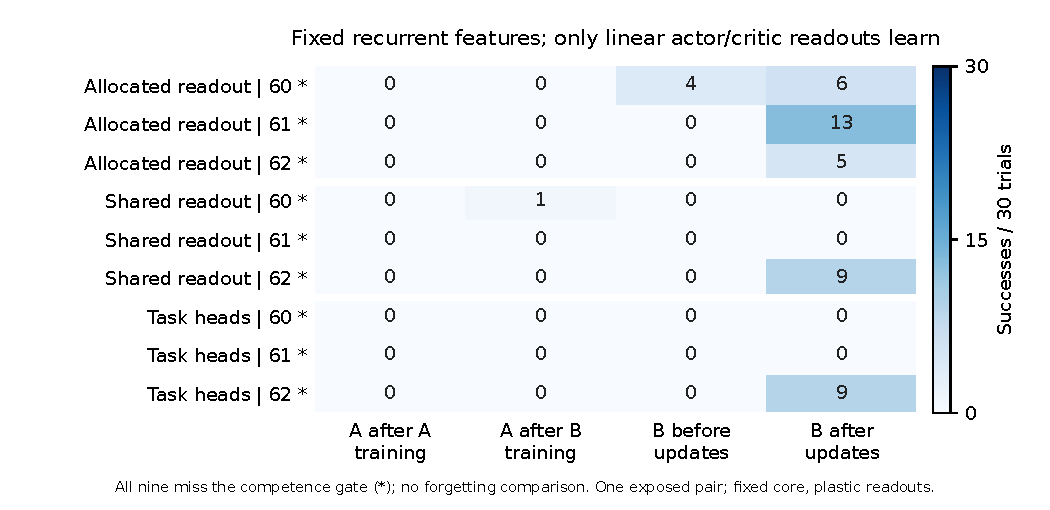
\includegraphics[width=.95\textwidth]{figs/fig_local_res_pilot.pdf}
\caption{\textbf{Fixed-feature local-readout control: acquisition failed.} All nine cases and all frozen
before/after probes. The pretrained FF branch and recurrent core remain fixed; only linear residual readouts
learn. Every $*$ marks a failed two-goal competence gate. A acquisition is not established, so zero-to-zero scores are not
competent retention. B-before probes use the actual B route, including the task-head copy. One exposed pair,
three seeds per arm; no conclusion about published biological learning methods.}
\label{fig:local_readout}
\end{figure*}
A separate registered extension fixes the FF branch and recurrent core in Section~\ref{sec:ffres_pilot},
training only the linear residual actor/critic readouts. Their gradients factor into presynaptic activity
and an output error: $\partial\mathcal L/\partial R=\sum_t g_t h_t^\top$, where $g_t$ contains the
clipped policy/entropy or value term. An analytic check agrees within $2.3\times10^{-16}$; the computational
graph has no hidden-layer or recurrent gradients. PPO/GAE, advantage normalization, 16-step rollouts,
minibatch reuse, Adam and global clipping remain. This is local linear-readout credit, not e-prop, local
recurrent-core learning, spiking or a biological online-learning demonstration.

The three arms are protected allocation (512 A units, 1,024 B units; A readout columns/biases frozen),
one unprotected shared readout, and separate task heads copied A-to-B. The last is expected to preserve
A structurally with fixed features; shared routing lacks this protection. Thus routing and active capacity
differ, and no contrast isolates locality. All nine fits use the same seeds, budgets and pretrained policy;
the driver, gates and independent auditor were bound before full fits, without retuning.

All arms fail the acquisition gate: A after A-training is 0/30 in every case. Allocated B scores are 6/13/5, shared 0/0/9 and
task-head 0/0/9 for seeds 60/61/62. These cannot establish catastrophic forgetting or protection of learned
competence (Fig.~\ref{fig:local_readout}). Independent replay checks all 810 primary episodes within
$1.2\times10^{-7}$ probability error and verifies every non-readout weight unchanged. All cases are preserved. A before-outcome diagnostic specifies all nine after-A checkpoints on B before B updates: allocated scores are 4/0/0, and both controls score 0/0/0. All 270 frozen episodes pass independent replay.
Readout weights changed and probe action entropy remained nonzero. This is an acquisition failure of this configuration, not a forgetting result or a test of published local rules. Relative to the successful recurrent pilot, both FF and core plasticity changed; their causal roles cannot be separated.

\section{Scope of local-learning development tests}
Our earlier local, spiking and remapping controllers were development adaptations without a native-benchmark
reproduction gate. They cannot support conclusions about the published methods or biological learning.
Their acquisition failures are not evidence of catastrophic forgetting: competence must first be established.
A backpropagation control in the same online learner also failed to acquire the first goal in all three seeds;
this prevents attributing that failure to locality alone, but does not identify its cause. The local-rate
representation control below is explicitly a custom continuation after a backpropagation warm start.

\section{Representation geometry, calibrated readout and acting}
\label{sec:supp_rosetta}
\begin{figure}[htbp]
\centering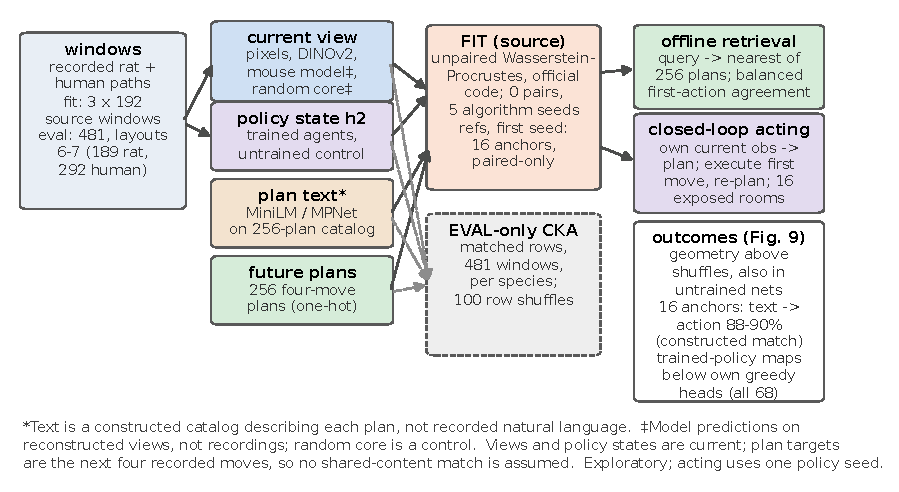
\includegraphics[width=.95\linewidth]{figs/fig_rosetta_pipeline.pdf}
\caption{\textbf{Rosetta pipeline (exploratory)}~\cite{schnaus2026rosetta}. Frozen vision and policy features encode current reconstructed observations;
action codes and generated language represent future four-move plans. Zero-pair fits use unpaired source clouds;
16-anchor and paired-only references calibrate correspondences. Matched held-out rows serve geometry/readout
evaluation. Acting queries the agent's own observations and replans the first move; recorded future actions
are never policy inputs. Mouse features are predictions; the random core retains trained readout, perspective
and modulation. The 88--90\% text/action result is balanced first-action agreement for constructed commands.
Results appear in main-paper Fig.~9; full controls follow below.}
\label{fig:supp_rosetta_pipeline}
\end{figure}
Figure~\ref{fig:supp_rosetta_pipeline} separates source fitting, geometric evaluation and acting.
\paragraph{Scope and event construction.}
This exploratory extension uses the same Tartarus release as the main paper. Cell-to-cell moves are grouped into
four-move windows with stride four, producing 5,674 windows. Each input contains the camera reconstructed from
the path prefix and public feedback; future actions provide evaluation targets, not policy inputs. Source layouts
1--5 supply three disjoint 192-window fitting clouds, each balanced at 96 rat and 96 human windows. Clouds and the
16 separate paired anchors share neither trials nor selected camera fingerprints. The evaluation set contains
481 windows from layouts 6--7 whose camera fingerprints do not occur in the selected fitting sets: 189 rat and
292 human windows, from three rats and six humans. The layouts and dataset had already been used in earlier
project evaluations, so this is not a new independent benchmark. Absent fitting fingerprints do not imply absence
from upstream encoder pretraining or the mouse-model source PCA.

\paragraph{Frozen representations.}
Pixel inputs have 144 dimensions. Predicted mouse and random-core features use the frozen source-fitted PCA144
from the main paper; the random core retains trained readout, perspective and modulation. DINOv2-B features
(768 dimensions) average the class and patch tokens after the final normalization~\cite{oquab2023dinov2}.
The released Hugging Face conversion is pinned; it is not a bitwise reproduction of the Rosetta authors'
TorchHub embedding files. The current 36$\times$64 reconstructed frame is replicated into RGB and resized to
224$\times$224 with bilinear antialiasing and ImageNet normalization. Generated instructions describe every one
of the $4^4=256$ cardinal plans. Frozen MiniLM-L6-v2 (384 dimensions) and MPNet-base-v2 (768 dimensions) encode
these instructions~\cite{wang2020minilm,song2020mpnet}. The action code concatenates four one-hot vectors
(16 dimensions, centred rank 12). Text is therefore a constructed common-content reference, whereas the current
image need not identify the future plan. No action-only foundation model is trained.

Policy representations are the fixed 64-dimensional second hidden layer. Rat-choice, human-choice, legal-label
and scratch policies have the shared 252-dimensional input contract and recorded source-training budgets.
Untrained policies use the same architecture and seeded initialization. Backpropagation and local-rate
continuations start from a rat-imitation/PPO warm start and receive 65,536 extra source frames at the fixed
learning rate .0003. The local arm uses fixed feedback and eligibility updates with Adam; it is not all-local
pretraining, a spiking network or a demonstrated memory-protection rule. The original plan-geometry diagnostic
exports three policy-training seeds per family; the completed alignment/acting comparison fixes policy seed 60.

\paragraph{Unpaired alignment and paired references.}
We use the authors' unmodified Wasserstein--Procrustes implementation~\cite{schnaus2026rosetta}, commit
\texttt{fdfad84ea488}, with 30 clusters, 30 restarts, batch size 10,000 and 100 refinement iterations. Source-only
centering and row normalization precede similarity scoring. Unequal-dimensional fits run from the lower- to the
higher-dimensional space; reverse retrieval transposes similarities rather than fitting an unsupported
high-to-low isometry. Five fixed author algorithm seeds are retained. The 16-anchor arm adds the fixed source
correspondences; the paired-only reference fits Procrustes to those same anchors without the unpaired step.
No anchor, direction relabeling, layer or best seed is selected from evaluation performance.

The prospective execution subset contains 132 primary jobs: 95 zero-pair, 19 fixed-first-seed 16-anchor and
18 paired-only references. Of these, 127 complete, two reach the registered 3,600-second cap, and three never
start because an SSH pre-authentication connection burst is rejected. All five statuses remain in the primary
results; incomplete five-seed groups have no mean (Fig.~\ref{fig:rosetta_retrieval_full}). The three never-started cases are completed once in a
separately registered recovery before the original deadline, without replacing primary records or entering the
acting study. An additional 49-job reference study completes all seven edges, each with five zero-pair seeds,
one 16-anchor fit and one paired-only fit. It includes DINOv2-to-action, MPNet-to-action, source-PCA64
DINOv2-to-MPNet, image-plus-past-to-text and text-plus-past-to-image, with matched past-only controls.
History features are strictly causal. Image retrieval scores equivalence classes of 116 distinct camera views,
not unique trajectory rows. Model versions, all configurations and the deferred jobs in the larger original plan
are included in the review code.

\paragraph{Pairwise geometry.}
After the original alignment/acting readout, we specify a separate descriptive all-pair analysis before computing
its new scores: 12 fixed spaces, 66 unordered pairs per species. The spaces are pixels, DINOv2, predicted mouse,
random core, MiniLM text, MPNet text, actions, human/rat/scratch/local policy states and the untrained policy.
Each uses its declared source-cloud mean and row L2 normalization; no whitening, clipping or new PCA is fitted.
Unbiased linear CKA is
\begin{equation}
\mathrm{CKA}(X,Y)=\frac{\langle\widetilde K_X,\widetilde K_Y\rangle_F}
{\|\widetilde K_X\|_F\,\|\widetilde K_Y\|_F},\qquad K_X=XX^\top,
\end{equation}
where $\widetilde K$ is the U-centred, zero-diagonal kernel. We retain every pair and all 100 fixed row-shuffle
values. The shuffle ranges are descriptive: correlated windows are not independent biological replicates.
The independent audit uses the alternative zero-diagonal Song HSIC formula. The earlier action-reference CKA
values reproduce within $1.5\times10^{-15}$. The earlier mutual-10NN diagnostic also retains its original tie
order: an independent implementation differs by at most one of 2,920 human neighbour overlaps, so fine model
rankings are not interpreted. Positive similarity, including that of untrained policies, does not establish
learned convergence or a brain mechanism.

\paragraph{From plan retrieval to action.}
Offline readout retrieves among all 256 plans. Similarities within $10^{-6}$ of the maximum share probability
uniformly; balanced first-action agreement averages within the four true first-action classes. It is not exact
four-move accuracy. Source-only modal-plan and previous-action references receive no held-out labels. The latter
achieves .388 rat and .409 human balanced agreement but only 1.67\% navigation success when executed online;
offline prediction and closed-loop competence are different endpoints. A relative $10^{-6}$ tie band changes
no top sets in any of the 176 completed primary/reference fits; the registered decision rule is unchanged.

The acting study retains 163 registered cases (Fig.~\ref{fig:rosetta_acting_full}): 158 complete and five lack their primary alignment dependency.
All completed cases use the same 16 exposed benchmark rooms, 30 trials per room, 45 decisions per trial,
fixed goal, policy seed 60 and evaluation seed 60. Maps receive the agent's own current observations and history,
not the recorded animal's counterfactual rewards or future plan. At each step they execute the first-action
distribution of the retrieved plans and replan. The primary comparator is the same policy's greedy native head;
sampled heads, mapped untrained features, uniform, persistence and source-mode actions are retained (Fig.~\ref{fig:rosetta_control_gaps}). Sensory-only
maps lack the policy's feedback and place belief and have no input-matched native head. A fixed 90-degree action
rotation is applied to the first algorithm seed only; it preserves similarities for the same observation, while
subsequent trajectories diverge. All 24 label-permutation oracle diagnostics are retained solely as diagnostics,
never used to choose, correct or report a favourable map.

\paragraph{Verification and reproducibility.}
All 127 completed primary and 49 reference metrics reproduce exactly from the stored similarities; native
float32 similarities reconstruct within $7.8\times10^{-7}$. Cross-host shared-input checks preserve every argmax
and tie set (map differences up to $3\times10^{-7}$); a remote parallel-restart bitwise-equality test fails and is
disclosed, but scientific fits use one worker and one thread. Two runtime audit-reader defects (obsolete gate
paths and a missing top-level seed alias on failed records) were repaired with original failures preserved;
scientific inputs, fits, statuses and decision rules were unchanged. Before acting, all 121 available real-map
readouts reproduce stored plan scores and tie sets. The independent acting audit checks 75,840 episodes and
3,216,202 decisions, including walls, rewards, path lengths, action probabilities and frozen model buffers.
Included CPU reanalysis recomputes all 132 pairwise CKAs from source-centred feature derivatives and navigation
rates/control differences from counts (290 checks). It does not rerun foundation encoders, optimization or
navigation. Full metrics and all incomplete cases accompany the figure sources.

\begin{figure}[p]
\centering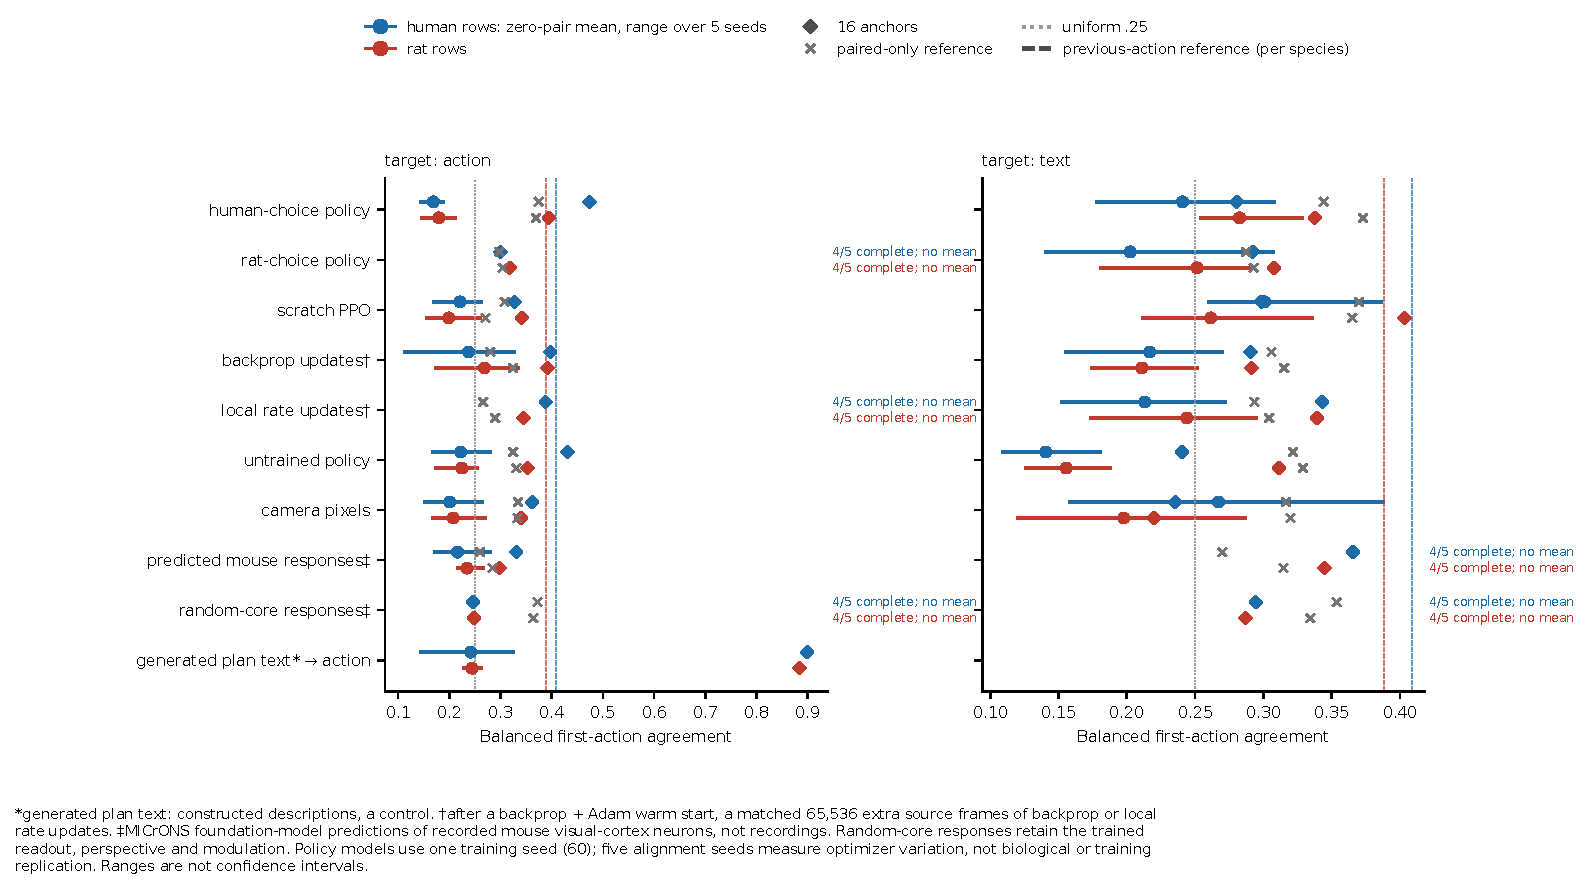
\includegraphics[width=\linewidth]{figs/fig_rosetta_retrieval_full.pdf}
\caption{\textbf{Complete offline action/text readouts.} All primary families, both recorded-species subsets,
zero-pair means and ranges only when all five algorithm seeds complete, fixed-first-seed 16 anchors and paired-only
references. Incomplete groups have no mean. Generated plan text is a constructed reference; cortical features
are predictions. Five alignment seeds are optimizer variation, not biological or policy-training replication.}
\label{fig:rosetta_retrieval_full}
\end{figure}
\begin{figure}[p]
\centering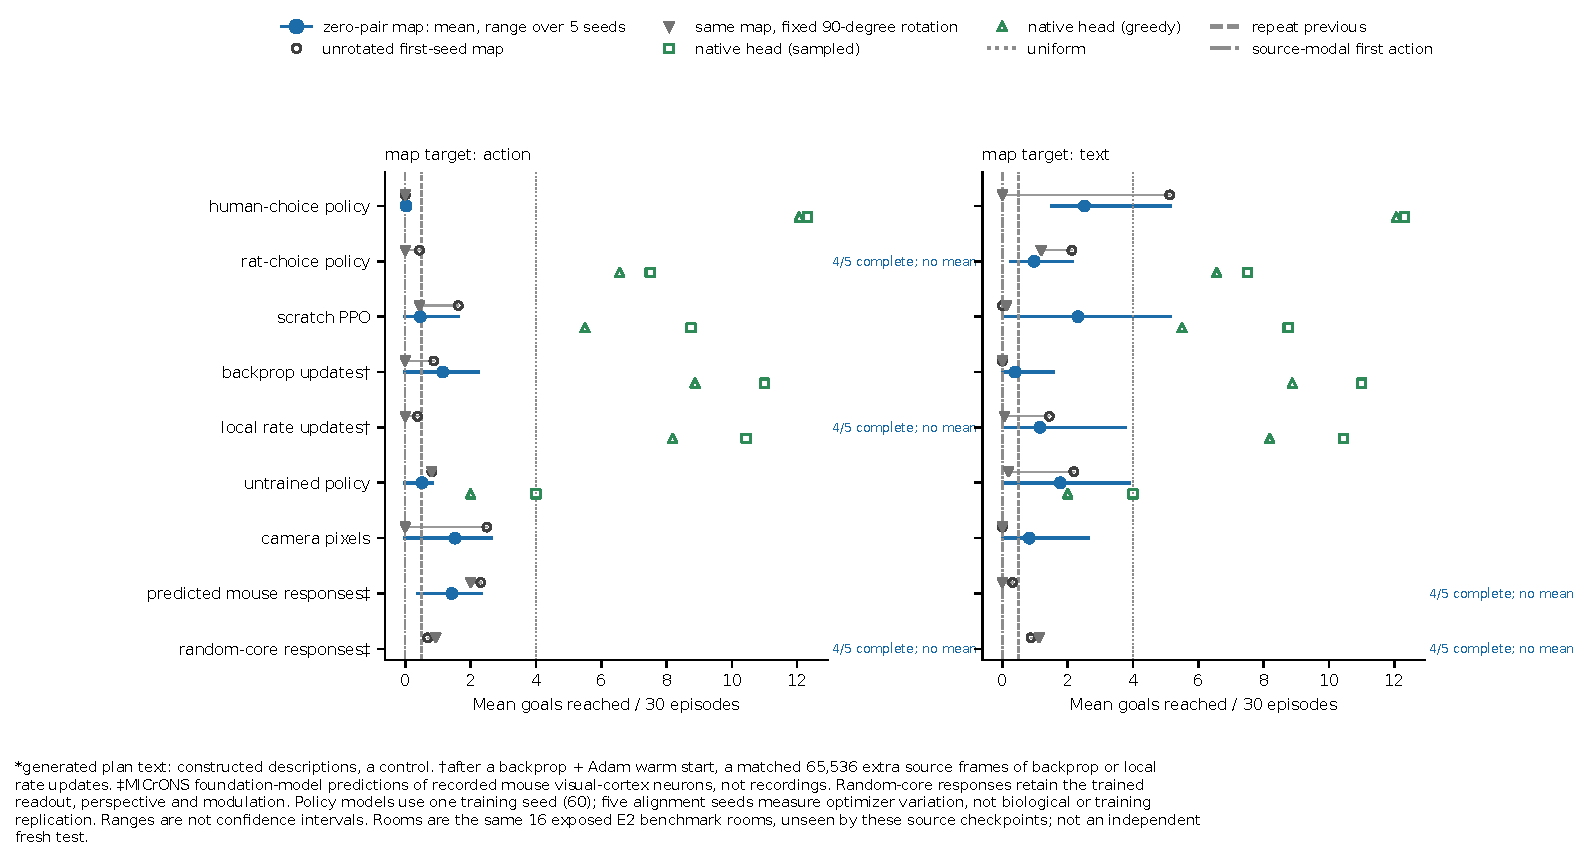
\includegraphics[width=\linewidth]{figs/fig_rosetta_acting_full.pdf}
\caption{\textbf{Complete unpaired acting readouts.} Action and generated-text targets in the same 16 exposed
rooms; one policy/evaluation seed. Own sampled and greedy heads are separate controls; fixed rotations are paired
with their own unrotated first-seed maps. The uniform line is 4/30 successes (13.3\%); the offline persistence
reference is a different metric. Sensory-only maps lack input-matched heads.}
\label{fig:rosetta_acting_full}
\end{figure}
\begin{figure}[p]
\centering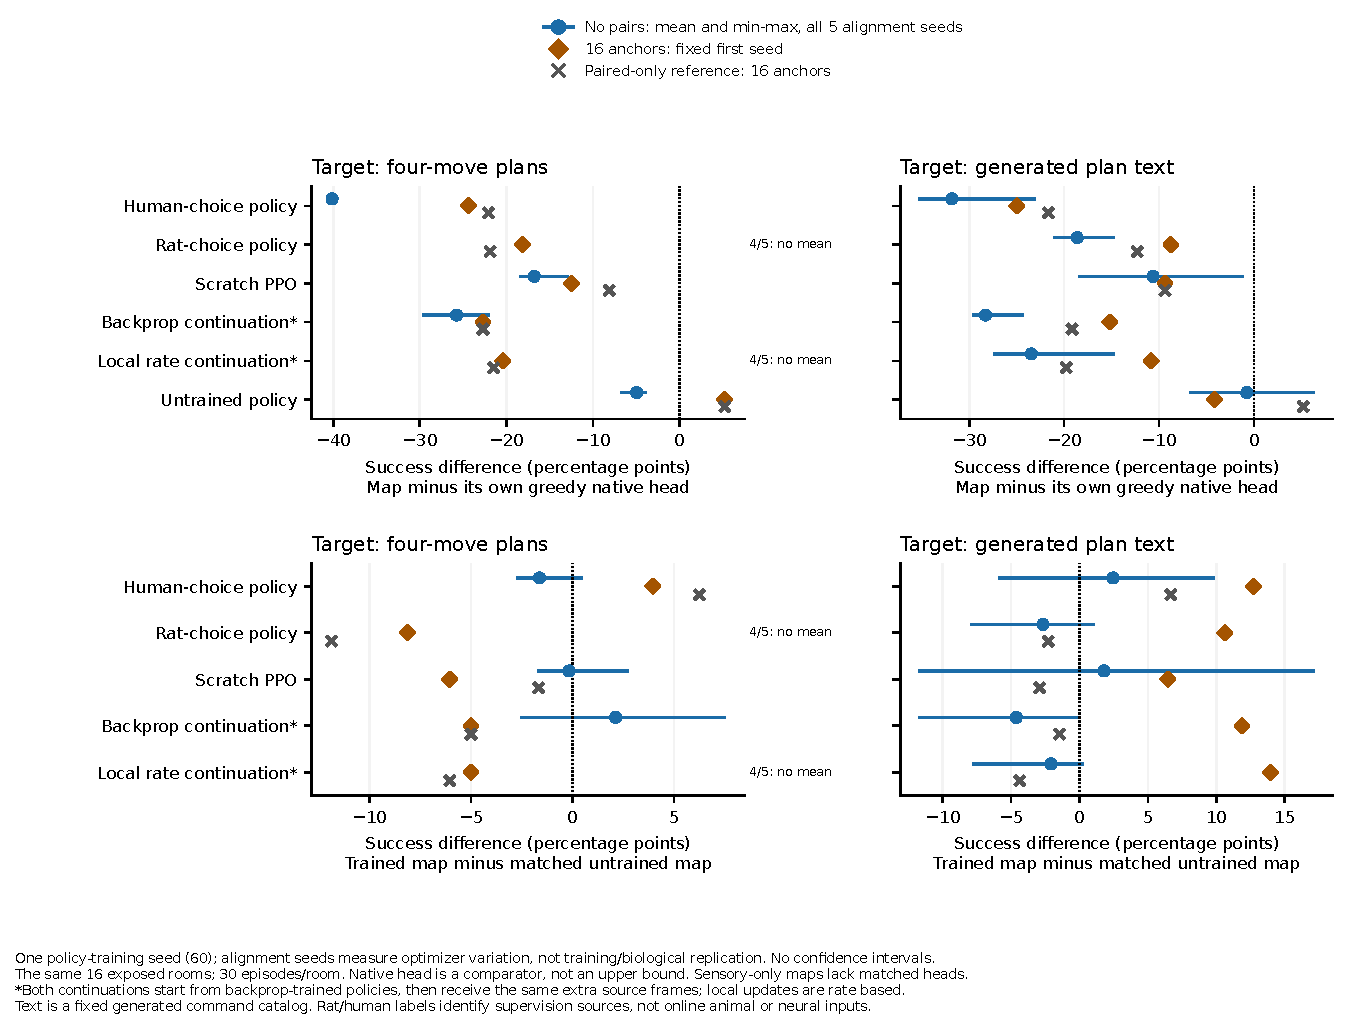
\includegraphics[width=\linewidth]{figs/fig_rosetta_control_gaps.pdf}
\caption{\textbf{Every calibrated control comparison.} Top: map minus its own greedy head. Bottom: trained-map
minus matched untrained-map, with the same target, alignment method, anchor count and algorithm seed. All 16-anchor
and paired-only comparisons are shown. Some calibrated maps improve over untrained maps; all evaluated
trained-policy maps remain below their own heads. Means and ranges are descriptive, not confidence intervals.}
\label{fig:rosetta_control_gaps}
\end{figure}

{\small
\bibliographystyle{ieeenat_fullname}
\bibliography{v4n_refs}
}

\section{Machine-checked statements (Lean 4)}
Lean checks the logic and arithmetic behind the claims, not the empirical effects (which are statistical
estimates). All statements build with \texttt{lake build} in \texttt{proofs/} (core Lean, no \texttt{sorry}, no added
axioms). \textbf{(i) Coverage} (\texttt{Claims.lean}, \texttt{relabel\_keeps\_states}): giving every recorded row a new
label leaves the sequence of states unchanged, so the legal-uniform control matches state coverage exactly.
\textbf{(ii) Paired contrast} (\texttt{paired\_sum}): the sum of per-seed differences equals the difference of sums.
\textbf{(iii) Species gap} (\texttt{species\_gap\_decomposition}): $H-R=(H_\ell-R_\ell)+((H-H_\ell)-(R-R_\ell))$,
with the reported $13.7=4.7+9.0$ pp. \textbf{(iv) Units}: 3 successes per 30 trials $=10$ pp.
\textbf{(v) Operation counts}: 20,544 dense multiply-accumulates per decision (4,416 hidden); spike-driven operations
are monotone in spike counts. \textbf{(vi) Loops} (\texttt{Loops.lean}), below.
With Mathlib (\texttt{proofs\_ml/ProofsML/Learning.lean}; only Lean's standard axioms \texttt{propext},
\texttt{Classical.choice}, \texttt{Quot.sound}): \textbf{(vii) the local readout rule is the exact policy gradient}
(\texttt{softmax\_logit\_grad}): $\partial\log\mathrm{softmax}_a(z)/\partial z_i=[i=a]-\mathrm{softmax}_i(z)$, so with
$z=Wh+b$ the TD-readout eligibility increment $(\mathbf{1}_a-\pi)h^\top$ is $\nabla_W\log\pi_a$; the TD error then
makes it an actor--critic update using only quantities local to each synapse plus one broadcast scalar.
\textbf{(viii) What the online trace computes} (\texttt{trace\_closed\_form}): $e_t=\gamma\lambda\,e_{t-1}+g_t$ equals
$\sum_{k\le t}(\gamma\lambda)^{t-k}g_k$. \textbf{(ix) Loops on finite states} (\texttt{orbit\_repeats}): a
deterministic orbit on a finite state space repeats within $|S|$ steps, so with (vi) a greedy agent on a finite state
space that has not reached the goal by then never will.
\textbf{(x) The circuit's trace is bounded} (\texttt{Trace.lean}, core Lean, \texttt{trace\_bounded}): with decay
$q=\gamma\lambda<1$ and inputs $|z|\le M$, every trace run from $|e|\le M/(1-q)$ stays there, so a value rate $\eta_v$
moves $V(s)$ by at most $\eta_v|\delta|M/(1-q)$ per step. The stage-3 search therefore samples the value rate in these
units, $\rho=\eta_v/(1-\gamma\lambda)$, which decouples it from $\lambda$ (stage-2 winners: $\rho=1.80$ and $0.70$).

\subsection{Greedy memoryless policies stay trapped}
\label{sec:lean}
With greedy (argmax) actions, the frozen network, the room, the renderer and the Bayes filter together define a
deterministic map $f$ on the complete state $s$ (cell, heading, last action, contact, reward, texture, posterior).
Let $f^{n}$ denote $n$ steps. \textbf{Lemma.} If $f^{i+p}(s)=f^{i}(s)$ for some $p>0$ and none of the $p$ states
$f^{i}(s),\dots,f^{i+p-1}(s)$ is a goal state, then $f^{i+n}(s)$ is not a goal state for any $n\ge0$.
The proof (every later state equals one of the $p$ cycle states, by induction on $n$) is checked in Lean~4 core
without axioms beyond the kernel: \texttt{proofs/Proofs/Loops.lean}, theorems \texttt{stays\_in\_cycle} and
\texttt{trapped\_forever}, built with \texttt{lake build}. No finiteness is assumed (the posterior is real-valued);
the lemma explains why greedy evaluation lowers every arm and why the registered probes sample actions.


\section{Joint-training reference for forgetting}
\label{sec:joint}
Reviewer 6g1M asked whether forgetting reflects sequential interference or a limit on doing both tasks at once, since a
feed-forward policy without a task signal receives identical inputs for two goals in one room. We registered
(\texttt{data/audit/v4n\_joint\_reference\_20261101}, before any outcome) a reference that keeps everything of the
moved-goal learning study (checkpoints, PPO and TD-readout with its frozen rate, room, 32,768 interactions, 30 seeds,
three priors) but alternates episodes between the moved goal and the familiar goal (3,3) in the same room (same walls,
same renders; the goal is invisible). An amendment fixed a bookkeeping error before any outcome was read.

\textbf{Aliasing.} From geometry alone, in 15.2\% of the trained rooms' cells (97 of 640) the shortest paths to the two
goals share no first move, so no goal-blind memoryless policy can be optimal for both there.

\begin{table}[h]\centering\small\setlength{\tabcolsep}{3pt}
\begin{tabular}{@{}llcc@{}}\toprule
learner & prior & joint: old / new goal & sequential: old / new\\\midrule
PPO & human choices & 88 / 44 & 32 / 61\\
 & human legal & 85 / 47 & 19 / 67\\
 & scratch & 79 / 47 & 22 / 54\\
TD-readout & human choices & 64 / 11 & 38 / 23\\
 & human legal & 60 / 19 & 24 / 36\\
 & scratch & 47 / 24 & 18 / 39\\\bottomrule
\end{tabular}
\caption{Success (\%) in the trained room after learning, 30 seeds per row.}\label{tab:joint}\end{table}

\textbf{J1 (supported).} Joint training retains the familiar goal far better: $+60.0$ pp ($[54.0,65.9]$) for PPO and
$+30.0$ pp ($[24.0,35.9]$) for TD-readout (Holm $p<10^{-15}$). \textbf{J2 (not supported).} We predicted that the summed
success would not exceed sequential learning (a capacity limit); instead it is higher by 45.0 pp ($[35.0,55.0]$) and
15.2 pp ($[8.6,21.8]$) (Holm $p\leq1.4\times10^{-5}$). The new goal is reached less often under joint training
($-15$ pp for both learners), which receives half the new-goal episodes. Reading: despite the aliasing, the same inputs
and network can hold both goals; the loss of the old goal after sequential learning is interference. Human-choice
priors again reach the new goal least under TD-readout, the inherited pull toward the old goal.

\section{Decision time and a learning control}
\label{sec:decision_time}
\textit{Registered 2026-10-31 before any outcome (\texttt{data/audit/v4n\_decision\_time\_20261031}); P1--P3 one Holm family.}
\textbf{Accumulate to bound.} Crow and primate choices stop when evidence accumulated over time reaches a
bound~\cite{schmidbauer2026crow}. Our spiking agents (Sec.~3.5) accumulate spikes; after each step $t$ the actor reads the
time-averaged spikes, and a decision stops at the first $t$ whose most likely action has probability $\ge\theta$
($\theta\in\{0.5,\dots,0.9\}$, at most 32 steps); the action is sampled as registered. Frozen source agents, familiar
goal, fresh rooms, 30 seeds.

\begin{table}[h]\centering\footnotesize\setlength{\tabcolsep}{3pt}
\begin{tabular}{@{}lrrrrrrrrr@{}}\toprule
 & \multicolumn{3}{c}{success (\%)} & \multicolumn{3}{c}{steps to decision} & \multicolumn{3}{c}{hidden ops / decision}\\
$\theta$ & human & legal & scratch & human & legal & scratch & human & legal & scratch\\\midrule
0.5 & 38.4 & 34.9 & 35.6 & 1.03 & 1.07 & 1.16 & 1,532 & 1,470 & 1,408\\
0.6 & 37.2 & 36.4 & 34.4 & 1.11 & 1.19 & 1.43 & 1,705 & 1,752 & 1,993\\
0.7 & 38.1 & 33.9 & 32.8 & 1.27 & 1.66 & 2.17 & 2,064 & 2,914 & 3,741\\
0.8 & 37.4 & 34.3 & 31.2 & 1.74 & 2.36 & 3.42 & 3,216 & 4,683 & 6,795\\
0.9 & 38.8 & 32.0 & 28.7 & 2.64 & 3.91 & 5.34 & 5,403 & 8,644 & 11,544\\
\bottomrule\end{tabular}
\caption{Accumulate-to-bound spiking decisions. Dense network: 4,416 hidden multiply-accumulates per decision.}\end{table}

\textbf{P1 (supported):} human-choice agents reach the bound in fewer steps than legal-label agents, $-0.48$ steps averaged
over $\theta$ ($[-0.73,-0.23]$, $p=.0004$). \textbf{P2 (not supported):} success $+3.7$ pp ($[-1.3,8.7]$, $p=.14$);
descriptively the gap grows with the bound ($+6.8$ pp, $[2.3,11.3]$ at $\theta=0.9$) because stricter bounds slow and
weaken the legal and scratch agents but not the human-choice agents. The first spiking step already gives the dense
network's choice in 69--76\% of decisions, the analogue of choice-predictive activity early in the trial. Faster
decisions here are a property of less ambiguous policies, not a claim about animal reaction times, which our data lack.

\textbf{P3: shuffled reward (supported).} TD-readout was retrained exactly as registered (30 seeds, 3 priors, same rate
and rooms) except that at every step the rewards of the 16 parallel rooms were permuted among them, keeping reward
statistics but breaking the action--reward contingency, as permuted decoding does for living neural
cultures~\cite{zhou2026embodied}. Final new-goal success fell from 23.4 to 8.6\% (human choices), 35.9 to 11.8\%
(legal) and 38.9 to 16.8\% (scratch); differences $+14.9$, $+24.1$, $+22.1$ pp, all $p<10^{-4}$.

\section{Matched-content image--text--action study}
\label{sec:rosetta_matched}
\textit{Registered 2026-10-31 before any outcome (\texttt{data/audit/v4n\_rosetta\_matched\_20261031}); answers reviewer 6g1M.}
In the reviewed version the text was generated from the action plan, so text--action similarity was circular. Here
image, text and action describe the same decision moment. \textbf{Image}: DINOv2-base on the rendered first-person
frame. \textbf{Text}: an exact description of what is visible, never of the action (``Ahead there is open floor. To the
left there is a drop with no floor. \dots\ The black curtain is to the right.''), embedded with MPNet.
\textbf{Action}: the frozen agent's own action probabilities. Moments: 40,000 decisions of frozen agents (4 priors
$\times$ 5 policy seeds) in the 16 fresh rooms; rooms 100--107 fit, 108--115 test.

\begin{table}[h]\centering\footnotesize\setlength{\tabcolsep}{3pt}
\begin{tabular}{@{}lrrrrrrrrrr@{}}\toprule
 & \multicolumn{3}{c}{B: predict the action (\%)} & \multicolumn{3}{c}{A: CKA} & \multicolumn{2}{c}{C: composed (\%)} & \multicolumn{2}{c}{D: closed loop (\%)}\\
prior & image & text & majority & img--txt & txt--act & img--act & img$\to$txt$\to$act & shuffled & composed & own head\\\midrule
human choices & 76 & 77 & 46 & 0.35 & 0.33 & 0.17 & 72 & 34 & 11.3 & 44.8\\
human legal & 74 & 69 & 48 & 0.35 & 0.30 & 0.14 & 67 & 39 & 12.8 & 37.8\\
rat choices & 79 & 78 & 44 & 0.34 & 0.38 & 0.16 & 70 & 46 & 9.5 & 33.4\\
scratch & 80 & 76 & 51 & 0.36 & 0.40 & 0.21 & 70 & 45 & 14.0 & 31.8\\
\bottomrule\end{tabular}
\caption{Matched content (5 policy seeds; held-out rooms). D: success of agents driven by the composed map versus the
same agents' own heads in the same rooms; uniform policy 13.3\%.}\end{table}

\textbf{Reading.} With matched content, a description of the view predicts the agent's next action far above the
majority baseline, and an image$\to$text map fitted on some policy seeds composes with a text$\to$action probe fitted on
other seeds to recover the action (67--72\% versus 34--46\% for a shuffled probe). Image, text and action are therefore
linked without circularity. Yet the composed map navigates at chance in closed loop, far below each agent's own head:
the view text carries no position or goal, which the agents take from their pose belief. Shared, predictive geometry is
not navigation competence.

\textbf{Lexical control.} The view text says ``to the left/right'' (egocentric) while the actions are named down, up,
right and left (allocentric moves), so the two share words. We reran A--D with the same content worded without any
action name (``In front \dots\ On the anticlockwise side \dots\ On the clockwise side \dots''; a check asserts that no
caption over every cell, heading and floor state contains an action word; amendment written before the rerun). The
predictive link is unchanged: text$\to$action 69--78\% (identical to within 1 pp for every prior), composed 68--71\%
versus 35--45\% shuffled, closed loop still at chance (10.5--16.2\%). The text--action CKA, by contrast, roughly halves
(0.17, 0.15, 0.31, 0.21 versus 0.33, 0.30, 0.38, 0.40): the geometry score depends on wording, the prediction does not.
We therefore base the linkage claim on prediction and composition, not on CKA.

The Rosetta paper's own protocol and code (their geometry scores, unpaired
Wasserstein--Procrustes alignment with 0 and 16 pairs, FOSCTTM; upstream tests 46/46 pass in our environment) are
applied to the same data (descriptive, secondary; 5 Rosetta seeds per cell; image--text on all rows, image/text--action
per prior; geometry on 1{,}000 held-out rows; amendment~4 fixed an index bug for cells with fewer rows, before any
outcome was seen). Their geometry scores reproduce the shared structure: unbiased CKA 0.32 for image--text, 0.28--0.41
for text--action and 0.14--0.23 for image--action, all against $\le$0.001 with rows shuffled; mutual $k$NN is small
everywhere (0.10 image--text, 0.016--0.026 with action, versus 0.007--0.022 shuffled). Their unpaired alignment does
\emph{not} recover which row matches which. With 0 known pairs, FOSCTTM (0.5 = chance, 0 = perfect) is 0.57 for
image--text and 0.50--0.53 for image--action, and 0.34--0.42 for text--action with a large seed spread (SD up to 0.17).
Sixteen known pairs help every pair (image--text 0.30, text--action 0.26--0.32, image--action 0.39--0.43), but the matching
remains far from perfect. Geometry that is shared on average is not enough, without pairs, to say which view goes with
which action. This is the same conclusion as the closed-loop test above.

\emph{Action-word-free captions (amendment~5, written before the rerun).} The same protocol, seeds and code were rerun
with the captions that never name an action. Image and action features are unchanged, and the 20 image--action jobs
reproduce the original values exactly (20/20 identical; a determinism check). Removing action words lowers text--action
CKA (0.16--0.31 versus 0.28--0.41) and moves unpaired text--action FOSCTTM to chance (0.47--0.55 versus 0.34--0.42;
below 0.5 in 10/20 jobs versus 18/20). The earlier better-than-chance unpaired matching came from wording that shares
words with the action names. Image--text gives CKA 0.23 (versus 0.32) and unpaired FOSCTTM 0.42 (versus 0.57); with 16
pairs, the values are 0.32 (image--text) and 0.34--0.42 (text--action). Mutual $k$NN does not change (0.10; 0.016--0.025).
Without lexical overlap, none of the three modalities can be matched to the actions without pairs. This agrees with the
main text: the views carry where the open paths are, while the choices carry the human content.

\emph{Where does the view determine the move? (amendment~6, descriptive, before computing.)} The same moments are
split by geometry. A move is \emph{forced} when one way other than back is open and a \emph{junction} otherwise. The
goal is never drawn, so ``goal near'' means it lies in an adjacent cell inside the visible range. Probes and the Rosetta
geometry scores are computed per stratum in the test rooms, pooled over arms (Table~\ref{tab:strata}). A ``goal-bearing''
caption adds where the goal lies and how far: it is what a view would say if the goal were visible. The text--action
geometry is strongest where the walls force the move. At junctions the view still predicts most moves, far above a uniform
choice among open ways, mostly through the curtain's bearing. When the goal is in the visible range, its bearing makes the
move near certain, and these moves are 93\% shortest-path. The view-based probe almost never predicts a move back (0--2\%
of moves, versus 1.6\% for the agents), so the closed-loop failure is not a failure to avoid going back. We do not identify
its mechanism here.
\begin{table}[h]\centering\small\setlength{\tabcolsep}{3pt}
\begin{tabular}{lrrrrrr}\toprule
stratum (share) & text & image & +goal & uniform & CKA$_{ta}$ & CKA$_{ia}$\\\midrule
forced (34\%) & .78 & .67 & .76 & .68 & .55 & .26\\
junction (58\%) & .79 & .79 & .73 & .35 & .29 & .13\\
junction, goal near (1\%) & .53 & .73 & .91 & .28 & .29 & .19\\\bottomrule
\end{tabular}
\caption{Action accuracy of the room-held-out probes and Rosetta CKA (text--action, image--action; shuffled $\le$0.01) per
stratum. Junction with the goal near: mutual $k$NN text--action 0.16 (shuffled 0.04). Per arm: human-choice moves are
the most predictable from the view at junctions (0.83, versus 0.76--0.80).}\label{tab:strata}
\end{table}

\section{Biologically plausible learners: stability, context and a brain-constrained circuit}
\label{sec:bio}
All studies here use the moved-goal protocol of the main text: 32,768 interactions, configurations chosen on development
rooms and seeds only, then tested once with 30 seeds $\times$ 3 priors in fresh rooms. Each probe uses 30 trials. Every
study was registered before its own outcomes (protocol, amendment and hash files in the audit folders). Contrasts are
paired by prior and seed, and the CIs are 95\%. Fig.~\ref{fig:tradeoff} plots every run in the keep--learn plane.

\paragraph{Search 2: replay and expansion (learn fast, forget).} The local rules of the main text were extended with
experience replay (GAE, clipped modulator, several epochs) and a fixed random $k$-WTA expansion (granule-like, 512--2048
cells, zero-initialised readout). Hidden credit comes from random feedback (DFA) or Error Diffusion routing; no learner
uses backpropagation. 160 TPE trials were run. The selected learners reach the new goal in almost every run (99.7--99.9\%,
versus PPO 61\%), and they reach it in the unseen room more often than PPO (40--47\% versus 28\%). They keep almost none of the old
goal (3\%, versus PPO 24\%). The human prior does not speed their learning (learning-curve area versus legal labels
$-3.8$ to $-2.2$ pp, Holm $p\geq.20$; head-only $-8.9$, Holm $p=.04$).

\paragraph{Why locality alone does not protect old skills.} Local rules are expected to change only the synapses a new task
uses. Here they move 52--94\% of the plastic synapses, so that expectation fails. Across all 810 learning runs,
old-goal success falls by 0.28 pp per pp of new-goal success, and at the same new-goal success local learners keep
7.6 pp less than PPO ($\pm$2.3, cluster-robust by seed). The two goals share their views and states, so a rule without a
context signal must overwrite the same synapses whatever its credit assignment. The joint-training reference
(Sec.~\ref{sec:joint}) shows that the network has room for both goals. Recent biologically plausible remedies all add a
signal that says \emph{when} or \emph{where} to learn: context-dependent gating~\cite{masse2018xdg}, evidence-gated
consolidation for multi-goal navigation~\cite{neymotin2026evidence}, astrocyte-like slow gates on
plasticity~\cite{dong2026astrocyte}, replay restricted to idle synapses~\cite{zhang2026silent}, and sparse fly-like
expansion codes~\cite{shen2023fly}. We tested the two families that need no task label.

\paragraph{Consolidation and old-goal replay (registered NSGA-II, 144 trials).} Each synapse is pulled back toward its
pre-learning value (a fast and a slow weight component~\cite{benna2016}). Before the switch, the frozen prior's own
familiar-goal experience is replayed between new chunks, counted inside the same budget (complementary learning
systems~\cite{mcclelland1995}). The best random-feedback learner (replay of 4,096 old frames, weak anchor) beats PPO on new-goal learning
($+17.1$ pp, $[9.3,24.9]$) and on the new goal in the unseen room ($+18.0$, $[12.6,23.5]$), and it keeps the old goal as
well as PPO ($+2.5$, $[-2.7,7.8]$). Against search 2, it trades 22 pp of new-goal success for 23 pp of retention. The
error-routing and head-only winners keep slightly less than PPO. With these learners the human prior no longer changes the
learning-curve area (Holm $p\geq.17$ for all six registered contrasts; point estimates $-4$ to $-14$ pp).

\paragraph{Context gating: forgetting is a missing context (registered, Holm over 4).} Only the expansion readout learns,
with the search-2 rule. G0 uses one code for all experience. G1 gives each goal its own half of the expansion (an oracle
upper bound). G2 has no cue: a latent-cause rule~\cite{gershman2010latent} switches halves when a CUSUM on episode outcomes
detects that the current context has stopped paying. Every condition learns the new goal (99.7--99.9\%). Old-goal
retention rises from 4.7\% (G0) to 57.5\% with the cue ($+52.8$ pp, Holm $p=10^{-33}$) and to 42.7\% when the context is
inferred ($+38.0$, $[33.5,42.4]$, Holm $p=10^{-29}$). Gating costs nothing on the new goal (G2$-$G0 $-0.04$ pp,
$[-0.36,0.29]$). In the unseen room G1 also keeps more of the old goal (36\% versus 8\%). The inferred-gate learner is
the only one here that keeps more of the old goal than PPO (43\% versus 24\%) while learning the new one fully.

\paragraph{Is the inference gap a tuning artefact? (registered NSGA-II, 160 trials; one test).} G2's runs switch
2.2$\times$ per old-goal probe, so we searched only its switch rule (establishment time, expectation floor, drop ratio,
CUSUM bound, dwell, reference cap) on dev rooms, with the learner, budget and rooms fixed. The best dev rule beat the
registered one there (54 versus 50\%) but not on the 30 test seeds in fresh rooms: old goal 40.0\% versus 42.7\%
($-2.7$ pp, $[-6.6,1.1]$, Holm $p=0.19$), new goal unchanged ($-0.2$ pp, $[-0.4,0.03]$), still $+35.3$ pp over the
ungated learner ($[30.3,40.2]$) and $-17.5$ pp under the cue ($[-22.0,-13.1]$). The registered rule is therefore near the
best of its family; the remaining gap to the oracle is the cost of inferring a hidden cause from outcomes alone, as
expected when both goals share views. Human choices again kept the most (50\% versus 35\% for legal labels and scratch).

\paragraph{A brain-constrained circuit (registered NSGA-II, 96 trials; descriptive test).} A mushroom-body /
cerebellum-like circuit sits on the frozen prior. It has sparse granule (Kenyon) cells, each wired to $c$ hidden
units~\cite{litwinkumar2017}, global inhibition (top fraction $f$) and divisive normalisation. Dopamine-like TD errors
gate an eligibility trace on the output synapses only (a three-factor rule~\cite{fremaux2016neuromodulated}). The circuit
also has metaplasticity, optional reverse replay of rewarded episodes and an optional inferred gate. It uses no batches,
no adaptive optimiser and no stored buffer, and it learns online. The selected circuit ($K$=4,096, $c$=7, $f$=3.5\%) keeps the
most of the old goal of any sequential learner (55\% versus PPO 24\%, $+31.0$ pp, $[24.5,37.4]$; unseen room 39\% versus
21\%). It also keeps more than the inferred-gate learner ($+12.4$ pp), with 29k synapses. It learns the new goal slowly
(15\% versus 61\%, $-45.5$ pp): it sits at the stable, slow end of the trade-off within this budget. The inferred gate
lowers both probes here ($-5.4$ and $-8.7$ pp). With this circuit, human-choice priors keep more of the old goal than
scratch priors ($+14.8$ pp, $[4.2,25.3]$).

\paragraph{Stage 2: awake replay lets the circuit learn (registered NSGA-II, 96 trials; one test).} Stage 1 learns
strictly online, whereas every learner here that learns the moved goal reuses each experience several times. Stage 2 keeps
the circuit and its rule and adds two mechanisms: after every $T$ steps the last $T$ steps are replayed $E$ times with the
same three-factor rule (awake sharp-wave-ripple replay of recent experience~\cite{foster2006reverse,ambrose2016reverse}), and,
optionally, the dopamine signal is divided by a slow running RMS of past TD errors (adaptive coding of prediction
errors~\cite{tobler2005adaptive}). The stage-1 winners, re-run inside stage 2, reproduce their dev scores exactly. Selected:
$K$=2,048, $c$=7; ungated $f$=5.5\%, $E$=8, $T$=16, adaptive dopamine; gated $f$=4.4\%, $E$=1, $T$=8. On the 30 test seeds
the ungated circuit learns the new goal in 60\% of runs (stage 1: 15\%) and is \emph{equivalent to PPO} in the trained room
within $\pm10$ pp (new goal $-0.6$ pp, $[-10.3,9.0]$, TOST $p=0.028$; old goal $+0.5$, $[-6.4,7.4]$, TOST $p=0.004$),
with 15k synapses and 113 active cells, no gradient through the prior, no adaptive optimiser, clipping or ratios, and no
divergence in 180 runs. With the inferred gate it keeps $+13.3$ pp more of the old goal than PPO ($[6.9,19.7]$) at
$-7.3$ pp on the new goal ($[-16.9,2.2]$), with 45 active cells. Replay buys learning at the price of retention
(old goal $-30.5$ pp versus stage 1, $[-36.4,-24.5]$): the same trade-off the gate and consolidation address. In the unseen
room it trails PPO on the new goal ($-7.9$ pp, $[-13.8,-2.1]$). Human-choice priors again help: versus scratch, $+15.9$ pp
on the new goal ($[0.1,31.6]$) and $+16.6$ on the old ($[6.2,26.9]$).

\paragraph{Stage 3: retuning in proved units beats PPO (registered NSGA-II, 120 trials on both GPUs; one test).} Stage 3
added sleep replay of stored old-goal episodes (interleaved replay~\cite{mcclelland1995}) and searched the value rate in
the units of the Lean trace bound (Sec.~\ref{sec:lean}, item x), $\rho=\eta_v/(1-\gamma\lambda)$, with $K$ and $c$ fixed.
Old-goal replay did not help on dev (best dev sum 34.3 without, 18.4--26.6 with) and both winners use none; the gated
winner is the stage-2 rule and reproduces its test exactly. The ungated winner ($f$=2.2\%, $\lambda$=.94, $\rho$=1.45,
$E$=4, $T$=16, adaptive dopamine, metaplasticity) learns the new goal in 73\% of test runs: $+12.4$ pp over PPO
($[3.8,21.1]$, $p=.006$) and $+13.1$ over stage 2 ($[4.5,21.6]$), while the old goal stays equivalent to PPO within
$\pm10$ pp ($+3.7$, $[-2.2,9.7]$, TOST $p=.019$); 0 of 90 runs diverged. In the unseen room it still trails PPO on the
new goal ($-7.4$ pp, $[-13.4,-1.5]$) and equals stage 2 there ($+0.5$, TOST $p<.001$). Human-choice priors learn the
new goal faster than scratch ($+16.2$ pp, $[2.1,30.3]$) but not than legal labels ($+7.4$, $[-6.9,21.8]$). The gain is
selection within a registered search, tested once; the stage-3 mechanism itself (old replay) was rejected.

\paragraph{Stage 4: a dense lateral-horn pathway is rejected (registered NSGA-II, 120 trials on one GPU; one test).}
Stage 4 targeted the unseen-room deficit. It added a dense, unit-normalised copy of the cortical input (gain $w$) to
the sparse code on the same output synapses, as the insect lateral horn runs parallel to the mushroom
body~\cite{litwinkumar2017}, and added the unseen-room new goal as a third dev objective. At $w=0$ the code
reproduces stage 3 exactly. Both dev winners use $w=0$, so the pathway was rejected. The gated winner is the stage-3 rule and reproduces
its test exactly. The ungated winner ($f$=2.2\%, $\lambda$=.83, $\rho$=1.99, $E$=4, $T$=8, adaptive dopamine) learns the
new goal in 75\% of test runs ($+14.6$ pp over PPO, $[5.9,23.4]$, $p=.001$). It keeps the old goal equivalent to PPO
($-1.4$, $[-7.6,4.7]$, TOST $p=.004$), and in the unseen room it no longer trails PPO significantly on the new goal ($-5.0$, $[-10.9,0.9]$,
TOST $p=.047$). It does trail on the familiar goal ($-7.2$, $[-11.5,-2.9]$). Against stage 3 the stage-4 winner is equivalent on
both new-goal probes (TOST $p\leq.016$) and lower on the familiar goal in the unseen room ($-4.9$, $[-8.7,-1.1]$). It is a fourth tested selection, so the main text keeps stage 3.

\paragraph{Stage 5: a proved transfer identity motivates a place drive, which is rejected (registered NSGA-II, 120 trials on one GPU; one test).}
For the three-factor update $\Delta W=\eta\,\delta\,g\,z_A^\top$ we prove in Lean~4 (Mathlib; \texttt{proofs\_ml/ProofsML/Transfer.lean},
standard axioms only) that the readout at any other state $B$ moves by exactly $\eta\,\delta\,g\,\langle z_A,z_B\rangle$. Transfer
to an unseen room is therefore proportional to code overlap. The same view in the trained and unseen rooms shares cosine .71 of its
Kenyon-cell code, versus .95 for PPO's learned hidden layer. The filter's place belief is room-invariant (cosine 1.00 along matched
paths). We also prove that a common drive $\beta c$ added to both pre-activations leaves their difference unchanged and raises
their inner product by $\beta(\langle a,c\rangle+\langle c,b\rangle)+\beta^2\|c\|^2$. Stage 5 therefore fed the 100-cell place belief to every Kenyon
cell through $c_p$ random synapses (gain $\beta\in\{0,.5,1,2,4\}$, $c_p\in\{3,7,15\}$), with the stage-4 objectives. One deviation
is disclosed: a probe-shape bug crashed every $\beta>0$ trial at the first launch, and it was fixed before any $\beta>0$ outcome
existed (ADDENDUM1). The ungated dev winner uses $\beta=0$, so the drive is rejected there. Its test is a new stage-3 configuration
that learns the new goal in 69\% of runs ($+8.1$ pp over PPO, $[-0.6,16.7]$). In the unseen room it reaches 23\% on the new goal
($-4.7$ vs PPO, $[-10.8,1.4]$, TOST $p=.044$; $+2.7$ vs stage 3, $[-2.0,7.5]$). The gated winner ($\beta=1$) keeps the old goal
better than PPO ($+12.3$, $[6.1,18.4]$) but falls to 11\% on the new goal in the unseen room ($-16.7$, $[-22.3,-11.2]$). Higher
overlap did not translate into transfer, so the result is a registered null; the main text keeps stage 3.

\paragraph{Stage 6: a context-gated goal-vector pathway removes most forgetting but not the unseen-room deficit (registered NSGA-II, 120 trials on one GPU; one test).}
Following central-complex models of vector memory, the readout also sees the place belief directly, $[z;\,g\,b]$ with
$g\in\{0,.1,.25,.5,1,2\}$; with the inferred gate each context writes its own copy of $b$. We prove in Lean~4 that the joined
code's overlap is $\langle z_A,z_B\rangle+g^2\langle b_A,b_B\rangle$ and that copies for different contexts are orthogonal, so
learning in one context cannot move the other context's place weights. Both dev winners use the pathway ($g=1$ ungated, $g=2$ gated).
On the test the gated circuit learns the new goal in 84\% of runs and still reaches the old goal in 58\%: $+22.9$ ($[15.0,30.8]$) and
$+33.6$ ($[26.1,41.0]$) over PPO, and $+30.3$ and $+20.3$ over gated stage 3. In the unseen room it reaches the new goal in only 7.5\%
($-20.3$ vs PPO, $[-25.7,-14.9]$; $-5.1$ vs stage 3). The ungated circuit learns 81\% ($+20.1$ vs PPO) but forgets (old goal 18\%) and
reaches 13\% in the unseen room ($-15.2$, $[-20.5,-9.8]$). The place pathway thus buys continual learning in the trained room and
costs transfer: a place-to-action map learned in one layout steers into walls in another. No configuration matches PPO in the unseen room.

\paragraph{Stage 7: a hippocampal goal map transfers to never-seen rooms (registered NSGA-II, 80 trials on one GPU; one test).}
Every agent's own place belief peaks on the true cell at every step in all 16 fresh rooms, so the deficit is not perception: stages
1--6 store the goal in view$\to$action associations, which are layout-specific. Mammals store goals on the hippocampal place
map~\cite{tolman1948,okeefe1978}, where place fields accumulate at rewarded places~\cite{hollup2001,dupret2010}, and read routes
out of it by recurrent propagation and replay~\cite{ponulak2013,pfeiffer2013}. Stage 7 adds this to the stage-6 circuit: a one-shot
dopamine-gated Hebbian write of the rewarded place (fixed place-field shape, as in behavioural-timescale plasticity~\cite{bittner2017}),
a recurrent wavefront value over the place-cell lattice~\cite{ponulak2013}, short-term depression of a link after a
bump~\cite{tsodyks1997}, and inhibition of a remembered goal that gives no reward (a dopamine dip at an omitted
reward~\cite{hollerman1998}, acting as inhibition of return on places~\cite{posner1984}); both reset every episode, and no synapse or
goal memory changes in the probes. Its drive, in steps to the goal, is added to the circuit's logits with gain
$\kappa$. We prove in Lean~4 (\texttt{Wavefront.lean}) that, in any layout, the wavefront has no local maximum away from a goal and
that climbing it reaches a remembered goal within $|S|$ steps. Two scaling choices were fixed on one dev smoke run before
registration (disclosed); one search worker was restarted after a transient checkpoint read (ADDENDUM1). On the test, the ungated
winner ($\kappa=50$) learns the new goal in 92\% of runs, keeps the old goal in 100\%, and reaches the new goal in the never-seen room
in 83\% ($+55.2$ pp over PPO, $[47.4,63.0]$; $+70.4$ over stage 6) and the old goal there in 73\% ($+51.9$). The registered ablation
without the two within-episode mechanisms falls to 8\% in the never-seen room ($-19.4$ vs PPO): transfer needs both the room-invariant
goal memory and online repair of the map, a within-episode memory the feed-forward PPO baseline does not have.
Scope (descriptive, after the test): what transfers is a goal place in the arena frame. In the fresh pairs the familiar goal is the
same cell in both rooms and the moved goal is the same cell (2 pairs) or one cell away (6 pairs). The goal map reaches it in
73\% and 86\% of these never-seen-room trials respectively (PPO 32\%, 27\%; stage 3 23\%, 20\%), so it is not replaying one
coordinate, but a goal far from any remembered place is outside this benchmark and would require search. Leakage control (same
15 agents, browser port): with the goal moved $\ge$4 cells from every remembered place the goal map succeeds in 3\% (PPO 4\%),
and 99.6\% when its memory is re-centred there, so nothing in the input reveals the goal; the belief's input (distal cue rows)
is identical across layouts. The old goal is kept because the map holds both goal places and inhibition of return tries the
other after an empty visit.

\paragraph{Stage 8: a dopamine dip at every visited place removes the remaining loops (registered, no search; one test).}
\emph{Diagnosis} (descriptive; the project page's step-exact port of the tested agents, seeds 1000--1004 $\times$ 3 priors, the
30-trial probe in each seed's trained and never-seen fresh room, both goals). The memoryless agents (frozen priors, PPO, the
stage-3 circuit) fail by pushing into a wall: at trapped steps the place belief is correct (100\%) while the habit's preferred move
is optimal in 2--25\% of steps with $p=0.74$--$0.95$, and 8--14 of the last 16 moves are bumps; no within-episode state can change
this (\texttt{trapped\_forever}). The stage-7 goal map still failed with the familiar goal in never-seen rooms (62\% in these 15
agents; 90\% of its failures were loops), and there the \emph{drive itself} asked for the bump: the chosen link was already
depressed (99\% of trapped steps), yet it was the drive's best move ($D_a=0$, $p_{\rm drive}=0.78$--$1.00$). A depressed link is
valued as staying, and the blurred goal field makes the agent's own cell a local maximum of $v$ next to a wall
($v_c=G_{e,c}\ge\gamma_h\,v$ of every open neighbour), so staying, i.e.\ bumping, is optimal and short-term depression, which only
closes links, cannot help. Stage 7 inhibited a place only when $G_e$ exceeded 70\% of its maximum (a searched threshold), never on
the blur around a goal; a rarer second case was a field peak written at a mis-estimated, unreachable cell. Tested at probe time with
the stage-7 weights, inhibition at every visited place in proportion to its expectation ($\theta=0$) raised the never-seen familiar
goal from 61.8\% to 100\%, left the other three probes unchanged (81.8$\to$84.4, 93.3, 100) and removed every loop (trapped failures
0\%; bumps per episode 14.7$\to$2.5). Alternatives tried there were worse or redundant: valuing a known collision at zero (91.1\%),
removing the field behind a bump (harmful, 29.6\% on the moved goal), and an oracle that pre-closes the three visible links (69.6\%):
the loop is not a perception failure. \emph{Brain basis.} A dopamine pause at an omitted reward scales with the expectation that
was violated~\cite{schultz1997,hollerman1998}; the stage-7 rule already computes this dip ($G_e\leftarrow G_e(1-K_\sigma(c))$,
with $K_\sigma(c)_c=1$ so a visit removes the expectation at that cell exactly) and acts as inhibition of return on
places~\cite{posner1984}; the 70\% threshold had no biological reading and is dropped. Lean~4 corollary
(\texttt{Visited.lean}, standard axioms): after the dip the visited cell is not a source, so by \texttt{wave\_ascent} some open
neighbour has strictly higher value: the drive can never prefer to stay at a visited cell. \emph{Test} (registered with the
diagnosis and predictions before any run; the whole learner re-run with $\theta=0$ in both stage-7 winners, nothing else changed;
with $\theta=0.7$ the script reproduces the stage-7 record exactly; 30 seeds $\times$ 3 priors, paired with stage 7). Ungated: new
goal 96.7\%, old goal 100\%, never-seen room new goal 88.8\% ($+5.7$ pp, $[0.4,11.1]$; PPO 27.8\%), never-seen room old goal
\textbf{100\%} ($+27.3$, $[21.4,33.3]$; excluding the five diagnosis seeds $+25.7$, $[19.3,32.2]$). Predictions: P1 ($\ge+20$ on
the never-seen old goal) and P3 (trained-room probes within $\pm5$: $+4.4$, $0.0$) met; P2 (never-seen new goal within $\pm5$)
exceeded in the favourable direction ($+5.7$). The gated winner does not share the gain (never-seen old goal $+6.5$, $[3.1,10.0]$;
never-seen new goal $-6.6$, $[-12.7,-0.4]$; its predictions not met), so the ungated circuit remains the one we report. Disclosed:
the rule was chosen after probe-time outcomes on five seeds, two of them test seeds (hence the 25-seed contrast); a dry run of the
registered analysis on 40 partial records per arm was seen before completion (ADDENDUM2); the Lean file was added after
registration (ADDENDUM1). The page's loop diagnostic (\texttt{site/test/loops.mjs}) and the probe-time scripts are in the study
folder.
\emph{What ``never seen'' means here, and what 100\% does not mean} (descriptive, after the test; \texttt{site/test/leakage.mjs},
\texttt{efficiency.mjs}). The goal is not new: the familiar goal is cell (3,3) in every room, and the moved goal of the never-seen
room lies 0--1 cells from the one learnt in the trained room (the registered mirror rule). What is new is the layout: each
never-seen room differs from its trained partner in 30--32 of 100 cells (disjoint wall sets), from every development, prior-training
and Tartarus layout in $\geq$15 cells, and no two of the 16 rooms coincide. Learning always happens in the trained room
(\texttt{room\_of}), probes run with frozen weights and never write the goal memory, and the belief filter starts uniform and reads
only the distal-cue rows, which are identical across rooms (maximum difference $0$); the floor rows differ (the adjacent walls are
visible, as they should be). Controls with the same 15 agents: a goal $\geq$4 cells from every remembered place is reached in 5.3\%
of trials (stage 3: 3.8\%, PPO: 4.2\%), 100\% when the memory is re-centred on it, 8\% with no memory; so the 100\% is the
remembered place reached through unknown walls, not a goal read from the input. Nor is it the shortest route: in never-seen rooms the
old goal is reached in $1.67\times$ the shortest path on average (median $1.42$; exactly shortest in 17\% of trials; 3 bumps per
episode), the moved goal in $4.1\times$ (search around the shifted place), against $1.14\times$ in the trained room; the longest
shortest path is 14 moves, and the budget is 45.

\paragraph{The same networks in the animals' own mazes (registered, descriptive; the paper's claims are unchanged).}
\emph{Shared Tartarus layouts.} Configurations 6--25 were walked by both species and seen by no network (imitation used
choices from 1--5). With each layout's own ten starts and no retraining, recorded humans reach the familiar goal within 45
moves in 97\% of trials and rats in 85\%. Frozen networks trained on human or rat actions reach it in 57\% and 55\%. After
learning the moved goal, PPO keeps 10\% (new goal 21\%), stage~3 16\% (17\%) and stage~7 66\% (70\%). Successful human-trained
paths are 1.32$\times$ the shortest (humans 1.26, rats 1.67); visited-cell distributions overlap the humans' with a
Bhattacharyya coefficient of 0.73 (human versus rat 0.94). One analysis fix (rat tracking cells on removed modules, starts
off the native set) was registered as an addendum before any agent metric.
\emph{Brain geometry on the same states.} We rebuilt two recorded mazes in our arena with the same renderer and moves: the
rat W-track (DANDI 000978; 8 rats, dorsal CA1 and prefrontal units) and the human virtual towns (Zenodo 8058006; 11 patients,
hippocampal iEEG; streets rasterized at $\sim$14 units per cell, overlap 0.66/0.55). Each recorded trial was replayed through
every network, so model and brain are compared at identical positions and headings. RSA between condition RDMs (rats: cell
$\times$ heading, 32--36 conditions; humans: cell, 19--36) is above permutation for all networks, but much of it is space: a
track-distance RDM alone gives $\rho$=0.29 (rats) and 0.28 (humans), against split-half ceilings of 0.90 and 0.55. After
partialling out space, heading and raw pixels, rat RSA is $\le$0.07 for every network (best CA1: trained on rat actions,
0.071$\pm$0.048), and human RSA is largest for the network trained on human actions (0.117$\pm$0.052; stage~3 0.107, stage~7
0.105, rat-trained 0.034). Post hoc, the human-trained minus rat-trained difference is $+0.084\pm0.048$ in human hippocampus
(9 of 11 patients) and points the other way in rat CA1 and PFC ($-0.015$ to $-0.027$, intervals include 0). The data come
from different tasks and recording methods, so this is a descriptive species-matched trend, not a test.
\emph{Open arenas (second registered study).} The same replay in two open arenas: humans navigating to remembered object
locations (OpenNeuro ds005522; 40 patients with medial-temporal or hippocampal contacts, bipolar iEEG) and rats foraging in an
open field (DANDI 000405; 5 rats, 115 sessions of entorhinal, pre- and parasubiculum units). Here neural geometry is mostly
space: the track-distance RDM gives $\rho$=0.26 (rats) and 0.22 (humans); the human split-half ceiling is only 0.04. Beyond
space, heading and pixels, every network adds little (partial $\rho$ 0.00--0.05). In rats, the imitation networks and both
brain circuits sit slightly above PPO (0.048--0.054 versus 0.018; $n$=5); in humans no family differs (0.02--0.04). One
analysis fix (rat sessions with a single active unit give an undefined RDM) was added after the first output and is disclosed.
\emph{Rosetta modalities against the brain.} On these replayed states the Rosetta modalities (image: DINOv2 view; text: MPNet
caption; each network's action probabilities and hidden layer) enter the same condition-RDM comparison as the recordings (Spearman
$\rho$, seeds then subjects averaged; space and heading partialled out; registered before this output, though brain--image/text
and brain--network values above had been seen). Too few conditions (13--36) remain for the unpaired solver, so this is geometry
only. Beyond space, every network's hidden layer is closer to human hippocampal geometry in the towns (0.04--0.12; human-trained
0.121) than the view (0.011) or caption ($-$0.001). In rat CA1 the view is as close (0.079) as most hidden layers (0.055--0.115),
in rat PFC the caption (0.095) is exceeded only by PPO after learning (0.148), and in both open arenas view and caption (0.03--0.09)
are as close as any network (0.02--0.05). Action probabilities are never closer than the hidden layer by more than 0.03
($-$0.04 to 0.07). Caption and view share geometry (0.33--0.59); each hidden layer shares more with its actions than with the view,
except the goal-map circuit, whose actions are driven by the place map.
The interactive matrices for every setting and network are on the project page.

\paragraph{Spiking cost of the learned networks.} The learned networks were converted to signed integrate-and-fire
networks exactly as the priors were (10 seeds $\times$ 3 priors, learned task, trained room). Conversion preserves
success at every $T$ (PPO 63--64\% versus 63\% dense; search 2 99.3--99.9\% versus 99.4--99.9\%). The expansion
costs operations: search-2 networks need 0.8--3.5M synaptic operations per decision at $T$=8--32, versus 24--100k for PPO
and TD-readout. Their dense equivalent is 153k multiply-accumulates, versus 21k. The brain-constrained circuit
has 29k synapses; 141 of its 4,096 granule cells (3.4\%) are active per decision, so its output stage needs about 0.7k operations.

\begin{figure}[h]\centering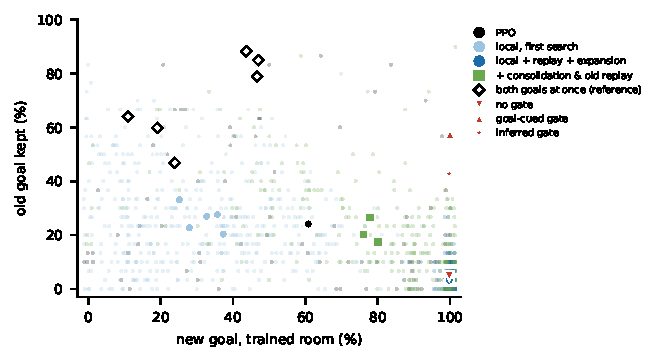
\includegraphics[width=\linewidth]{figs/fig_tradeoff.pdf}
\caption{Keep versus learn for every learning run (dots) and learner means (markers): PPO, local rules of the main text,
search 2, consolidation with old replay, context gating (red) and the joint-training reference (diamonds).}
\label{fig:tradeoff}\end{figure}
\begin{figure}[h]\centering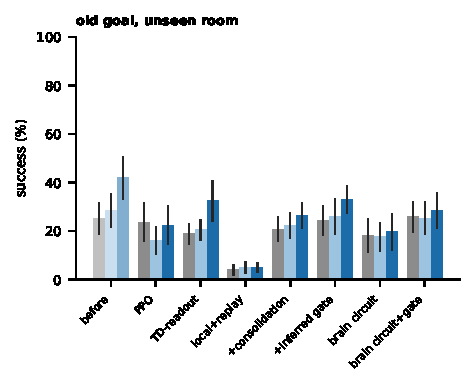
\includegraphics[width=.8\linewidth]{figs/fig_kpi_old_unseen.pdf}
\caption{Old goal in the unseen room after learning, per learner and prior (learners of the main-text four-claims figure).}\end{figure}

\section{Rosetta geometry across brains, priors and learners}
\label{sec:rbrains}
The Rosetta geometry scores~\cite{schnaus2026rosetta} (upstream code, unmodified) were computed between the hidden layer
of every network and each modality of the matched-content moments. The modalities are the image, the text, the predicted
mouse cortex (144 PCs and all 9,941 units) and the action. Networks were also compared with each other, all on
the same 1,000 held-out moments per job. There are 3 policy seeds $\times$ 3 Rosetta seeds, and shuffled controls are
$\le$0.01 everywhere (Fig.~\ref{fig:rbrains}). These analyses are descriptive. \emph{Schedule deviation:} the geometry
scores were computed first in one pass, with code identical to the registered jobs; the 882 WassersteinProcrustes
retrieval jobs finished afterwards (FOSCTTM on held-out moments; 0.5 is chance, lower is better).
\textbf{Retrieval.} Without pairs, modality-to-modality retrieval is at chance for image, text, cortex and action
(0.43--0.67), so the shared geometry does not identify individual moments; 16 pairs bring every pair to 0.12--0.47
(hidden$\to$action 0.12--0.28, cortex$\to$hidden 0.19--0.28, image$\to$action 0.42--0.47). The three-way bridge
(image or cortex $\to$ text $\to$ action, unpaired) is no better than the direct map (0.46--0.53 versus 0.48--0.63).
Between networks, however, unpaired alignment works when the training choices are shared, as in brain-to-brain
alignment: human-choice networks of different seeds 0.06; human choices versus legal labels 0.31; versus rat choices
0.59 and scratch 0.50 (chance). Learning keeps a network alignable with its prior (PPO 0.20, local rule 0.32; with 16
pairs 0.11 and 0.06). The choices, not the views, set the network geometry (``same views, different choices'' in the main text).
\textbf{PCA.} CKA between the 144-PC and the full cortex code is 1.00, and every comparison gives the same CKA with
either code. Only local neighbourhoods differ (mutual $k$NN between the codes is 0.36), so the reduction keeps the
geometry the main text uses. \textbf{Brains.} Text describing the view shares more geometry with the predicted cortex
than pixels do (0.51 versus 0.19). Hidden layers trained on human choices are closer to the cortex (0.49) than those
trained on rat choices or legal labels (0.40) or from scratch (0.44). \textbf{Networks.} Human-choice networks from
different seeds share most of their geometry (0.82--0.88). A human-choice network shares less with a rat network (0.58--0.71),
with a legal-label network (0.50--0.70) or with a scratch network (0.47--0.57). Learning a new goal keeps most of
it, with PPO (0.65--0.80) and with local rules (0.77--0.88). TD-readout leaves the hidden layer unchanged, a
built-in check. With the expansion, the action is read from new cells, and hidden--action CKA falls from 0.58 to
0.23--0.31.
\begin{figure}[h]\centering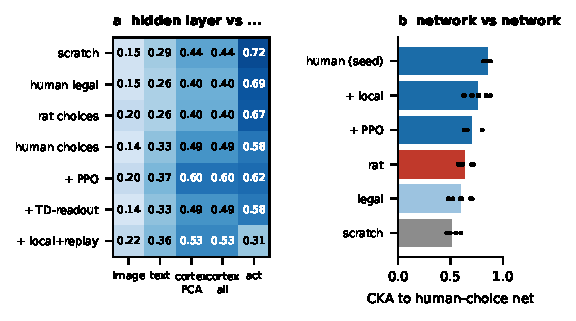
\includegraphics[width=\linewidth]{figs/fig_rosetta_brains.pdf}
\caption{Rosetta CKA. \textbf{a}~Hidden layer versus image, text, predicted cortex (PCA and all units) and action; rows
are priors and learners started from human choices. \textbf{b}~Hidden layer versus the human-choice network (dots: jobs).}
\label{fig:rbrains}\end{figure}

\end{document}
